% Seminarul 15: Recapitulare și pregătire pentru examen
% Serii de timp -- Programele de licență Informatică economică și Cibernetică economică, Academia de Studii Economice din București
% GENERAT de latex/build_seminar15.py -- modificați generatorul, nu acest fișier.
% Implicit versiunea pentru studenți; versiunea profesorului este wrapper-ul *_solutions.tex.
\makeatletter\@ifundefined{ifsolutions}{\expandafter\newif\csname ifsolutions\endcsname}{}\makeatother

\newcommand{\coursename}{Serii de timp}
\def\tsalang{ro}
% Preambul comun TSA -- Serii de timp / Time Series Analysis (Beamer, 16:9)
% Același design ca MFM și SFM (preluat din SFM, 5 octombrie 2026). Înainte de % Preambul comun TSA -- Serii de timp / Time Series Analysis (Beamer, 16:9)
% Același design ca MFM și SFM (preluat din SFM, 5 octombrie 2026). Înainte de % Preambul comun TSA -- Serii de timp / Time Series Analysis (Beamer, 16:9)
% Același design ca MFM și SFM (preluat din SFM, 5 octombrie 2026). Înainte de \input{../../latex/preamble} se definește
%   \newcommand{\coursename}{Time Series Analysis}      (EN)
%   \newcommand{\coursename}{Serii de timp}       (RO)  și  \def\tsalang{ro}
% Fișierele .tex se află în EN/Courses, EN/Seminars, RO/Cursuri, RO/Seminarii (două niveluri sub rădăcină).
% Deck-urile sînt generate de latex/build_chapterN.py / build_seminarN.py (vezi latex/tsa_build.py).

\documentclass[9pt, aspectratio=169, t]{beamer}
\providecommand{\coursename}{Time Series Analysis}

% Ensure content fits on slides
\setbeamersize{text margin left=8mm, text margin right=8mm}
% Smaller institute font (title page)
\setbeamerfont{institute}{size=\footnotesize}

%=============================================================================
% THEME AND STYLE CONFIGURATION
%=============================================================================
\usetheme{default}
% Using default theme for clean header/footer control

% Color Palette (matching Redispatch PDF)
\definecolor{MainBlue}{RGB}{26, 58, 110}
\definecolor{AccentBlue}{RGB}{26, 58, 110}
\definecolor{IDAred}{RGB}{205, 0, 0}
\definecolor{DarkGray}{RGB}{51, 51, 51}
\definecolor{MediumGray}{RGB}{128, 128, 128}
\definecolor{LightGray}{RGB}{248, 248, 248}
\definecolor{VeryLightGray}{RGB}{235, 235, 235}
\definecolor{KeynoteGray}{RGB}{218, 218, 218}
\definecolor{SectionGray}{RGB}{120, 120, 120}
\definecolor{FooterGray}{RGB}{100, 100, 100}
\definecolor{Crimson}{RGB}{220, 53, 69}
\definecolor{Forest}{RGB}{46, 125, 50}
\definecolor{Amber}{RGB}{181, 133, 63}
\definecolor{Orange}{RGB}{230, 126, 34}
\definecolor{Purple}{RGB}{142, 68, 173}

% Gradient background (exact Keynote 315° gradient: white to RGB 218,218,218)
\setbeamertemplate{background}{%
    \begin{tikzpicture}[remember picture, overlay]
        \shade[shading=axis, shading angle=315,
        top color=white, bottom color=KeynoteGray]
        (current page.south west) rectangle (current page.north east);
    \end{tikzpicture}%
}
% Fallback solid color for compatibility
\setbeamercolor{background canvas}{bg=}

\setbeamercolor{palette primary}{bg=MainBlue, fg=white}
\setbeamercolor{palette secondary}{bg=MainBlue!85, fg=white}
\setbeamercolor{palette tertiary}{bg=MainBlue!70, fg=white}
\setbeamercolor{structure}{fg=MainBlue}
\setbeamercolor{title}{fg=IDAred}
\setbeamercolor{frametitle}{fg=IDAred, bg=}
\setbeamercolor{block title}{bg=MainBlue, fg=white}
\setbeamercolor{block body}{bg=VeryLightGray, fg=DarkGray}
\setbeamercolor{block title alerted}{bg=Crimson, fg=white}
\setbeamercolor{block body alerted}{bg=Crimson!8, fg=DarkGray}
\setbeamercolor{block title example}{bg=Forest, fg=white}
\setbeamercolor{block body example}{bg=Forest!8, fg=DarkGray}
\setbeamercolor{item}{fg=MainBlue}

% Footer colors (override Madrid theme blue)
\setbeamercolor{author in head/foot}{fg=FooterGray, bg=}
\setbeamercolor{title in head/foot}{fg=FooterGray, bg=}
\setbeamercolor{date in head/foot}{fg=FooterGray, bg=}
\setbeamercolor{section in head/foot}{fg=FooterGray, bg=}
\setbeamercolor{subsection in head/foot}{fg=FooterGray, bg=}

% Bullet styles (apply everywhere including blocks)
\setbeamertemplate{itemize item}{\color{MainBlue}$\boxdot$}
\setbeamertemplate{itemize subitem}{\color{MainBlue}$\blacktriangleright$}
\setbeamertemplate{itemize subsubitem}{\color{MainBlue}\tiny$\bullet$}
\setbeamertemplate{itemize/enumerate body begin}{\normalsize}
\setbeamertemplate{itemize/enumerate subbody begin}{\normalsize}

% Item spacing - compact style
\setlength{\leftmargini}{10pt}       % Level 1: minimal indent
\setlength{\leftmarginii}{10pt}      % Level 2: minimal additional indent
% Compact list spacing (zero extra space before/after lists in blocks)
\makeatletter
\def\@listi{\leftmargin\leftmargini \topsep 0pt \parsep 0pt \itemsep 0pt}
\def\@listii{\leftmargin\leftmarginii \topsep 0pt \parsep 0pt \itemsep 0pt}
\makeatother

\setbeamertemplate{navigation symbols}{}

%=============================================================================
% CUSTOM HEADLINE
%=============================================================================
\setbeamertemplate{headline}{%
    \vskip10pt%
    \hbox to \paperwidth{%
        \hskip0.5cm%
        {\small\color{FooterGray}\renewcommand{\hyperlink}[2]{##2}\insertsectionhead}%
        \hfill%
        \textcolor{FooterGray}{\small\insertframenumber}%
        \hskip0.5cm%
    }%
    \vskip4pt%
    {\color{FooterGray}\hrule height 0.4pt}%
}

%=============================================================================
% CUSTOM FOOTER
%=============================================================================
\usepackage{fontawesome5}

\setbeamertemplate{footline}{%
    {\color{FooterGray}\hrule height 0.4pt}%
    \vskip4pt%
    \hbox to \paperwidth{%
        \hskip0.5cm%
        \textcolor{FooterGray}{\small\coursename}%
        \hfill%
        \raisebox{-0.1em}{%
            \begin{tikzpicture}[x=0.08em, y=0.08em, line width=0.4pt]
                \draw[FooterGray] (0,3) -- (1,4) -- (2,3.5) -- (3,5) -- (4,4) -- (5,6) -- (6,5.5) -- (7,4) -- (8,5) -- (9,7) -- (10,6) -- (11,5) -- (12,6.5) -- (13,8) -- (14,7) -- (15,6) -- (16,7.5) -- (17,9) -- (18,8) -- (19,7) -- (20,8.5) -- (21,10) -- (22,9) -- (23,8) -- (24,9.5);
            \end{tikzpicture}%
        }%
        \hskip0.5cm%
    }%
    \vskip6pt%
}

%=============================================================================
% PACKAGES
%=============================================================================
\usepackage[utf8]{inputenc}
\DeclareUnicodeCharacter{03B1}{\ensuremath{\alpha}}
\usepackage[T1]{fontenc}
\usepackage{amsmath, amssymb, amsthm}
\usepackage{mathtools}
\usepackage{bm}
\usepackage{tikz}
\usetikzlibrary{arrows.meta, positioning, shapes, calc, decorations.pathreplacing, shadings}
\usepackage{booktabs}
\usepackage{multirow}
\usepackage{array}
\usepackage{graphicx}
\usepackage{animate}
\usepackage{hyperref}
\usepackage{colortbl}
\usepackage{listings}
\lstset{language=Python, basicstyle=\ttfamily\scriptsize, keywordstyle=\color{MainBlue}\bfseries,
  commentstyle=\color{Forest}, stringstyle=\color{Crimson}, breaklines=true,
  frame=none, backgroundcolor=\color{VeryLightGray}, xleftmargin=2mm}
\hypersetup{colorlinks=true, linkcolor=MainBlue, urlcolor=MainBlue}
\graphicspath{{../../logos/}{../../charts/}{../../photos/}}
\usepackage{xcolor}
\hfuzz=2pt  % Suppress tiny overfull warnings (<2pt)
\vfuzz=2pt  % Suppress tiny vertical overfull warnings (<2pt)
% \mathrm in the sans-serif family of the slides (beamer resets \mathrm to the serif family at \begin{document};
% this hook runs after beamer's, so WN, Var, RMSE, ... in formulas match the surrounding text)
% Bold vectors and matrices in the same sans-serif family: \mathbf{A} in sans bold (beamer's own \mathbf came out in
% medium weight), and the bold upright Greek capitals of \boldsymbol / \bm (\bSigma, \bPhi, \boldsymbol{\Theta}) in
% cmss bold: bm.sty fixes its "boldoperators" font when it is loaded (serif cmbx), before beamer switches the
% operators to cmss, so it is reset here.
\AtBeginDocument{%
  \SetMathAlphabet{\mathrm}{normal}{\encodingdefault}{\sfdefault}{\mddefault}{n}%
  \SetMathAlphabet{\mathrm}{bold}{\encodingdefault}{\sfdefault}{bx}{n}%
  \SetMathAlphabet{\mathbf}{normal}{\encodingdefault}{\sfdefault}{bx}{n}%
  \SetMathAlphabet{\mathbf}{bold}{\encodingdefault}{\sfdefault}{bx}{n}%
  \SetSymbolFont{boldoperators}{normal}{OT1}{cmss}{bx}{n}%
  \SetSymbolFont{boldoperators}{bold}{OT1}{cmss}{bx}{n}}

%=============================================================================
% QUANTLET COMMANDS
%   \quantlet{<displayed name>}{<url>}       (generic, compatible with the older TSA decks)
%   \tsaquantlet{Ch_05}{TSA_ch5_garch}       -> https://github.com/danpele/Time-Series-Analysis/tree/main/Quantlets/Ch_05/TSA_ch5_garch
%   \qlurl{<folder>} is defined per chapter by the generator (Quantlets/Ch_NN/<folder>)
%=============================================================================
\newcommand{\tsarepo}{https://github.com/danpele/Time-Series-Analysis}
\newcommand{\tsaqlbase}{https://github.com/danpele/Time-Series-Analysis/tree/main/Quantlets}
\newcommand{\quantlet}[2]{%
    \hfill\href{#2}{%
        \raisebox{-0.15em}{
\includegraphics[height=0.7em]{ql_logo.png}}%
        \textcolor{MainBlue}{\tiny\ #1}%
    }%
}
\newcommand{\tsaquantlet}[2]{\quantlet{\detokenize{#2}}{\tsaqlbase/#1/#2}}

%=============================================================================
% NOTEBOOKS (Google Colab)
%   \colaburl{notebooks/EN/chapter5_seminar_notebook.ipynb} -> the Colab link of a file in the TSA repo
%   \nb: the chapter notebook (each seminar deck redefines it with \renewcommand)
%=============================================================================
\newcommand{\colaburl}[1]{https://colab.research.google.com/github/danpele/Time-Series-Analysis/blob/main/#1}
\newcommand{\nb}{https://colab.research.google.com/github/danpele/Time-Series-Analysis/tree/main/notebooks/EN}
\newcommand{\nbname}{notebooks/EN}

%=============================================================================
% SLIDE HELPERS (used by the generators; the same as in MFM)
%=============================================================================
% local font size for list bodies (the preamble forces \normalsize)
\newcommand{\itemsize}[1]{\setbeamertemplate{itemize/enumerate body begin}{#1}\setbeamertemplate{itemize/enumerate subbody begin}{#1}}
\newcommand{\intitle}[1]{{\hypersetup{urlcolor=white}#1}}   % white links inside coloured title bars
\newcommand{\imgcap}[1]{{\scriptsize #1}\\[0.5mm]}          % caption under a photo
\newcommand{\imgcredit}[2]{{\tiny\color{FooterGray}\href{#1}{#2}}}   % image credit: source URL, author/licence
\newcommand{\aiprompt}[1]{{\ttfamily\color{MainBlue}#1}}     % a prompt to an AI assistant

%=============================================================================
% SEMINARS: student version by default; the instructor wrapper *_solutions.tex sets \solutionstrue
%=============================================================================
\makeatletter\@ifundefined{ifsolutions}{\expandafter\newif\csname ifsolutions\endcsname}{}\makeatother
\newcommand{\solonly}[1]{\ifsolutions #1\fi}
\newcommand{\propsub}{\ifsolutions\else\framesubtitle{\ifdefined\tsalang Rezolvarea se discută la seminar\else Solution discussed in class\fi}\fi}

%=============================================================================
% APPENDIX AND CHAPTER LINKS (latex/appendix_links.py writes the calls; it also re-declares these
% macros before \begin{document}, so the decks compile with or without this preamble block)
%=============================================================================
\providecommand{\tsaapplink}[3]{\hypertarget{#2}{}\hyperlink{#1}{\beamergotobutton{#3}}}
\providecommand{\tsaappback}[2]{\begin{tikzpicture}[remember picture,overlay]\node[anchor=south east] at ([xshift=-3mm,yshift=7mm]current page.south east){\hyperlink{#1}{\beamerreturnbutton{#2}}};\end{tikzpicture}}
\providecommand{\tsachlink}[2]{\href{#1}{#2}}
\providecommand{\tsachlinkt}[2]{\href{#1}{\usebeamercolor[fg]{frametitle}#2}}

%=============================================================================
% QUANTINAR COMMAND: link către un curs Quantinar (subiecte avansate)
%=============================================================================
\newcommand{\quantinar}[2]{%
    \href{#2}{%
        \raisebox{-0.15em}{
\includegraphics[height=0.8em]{qr_logo.png}}%
        \textcolor{MainBlue}{\scriptsize\ #1}%
    }%
}

%=============================================================================
% CUSTOM TITLE PAGE
%=============================================================================
\defbeamertemplate*{title page}{hybrid}[1][]
{
    \vspace{0.2cm}
    % Logos row - top header (with clickable links)
    \begin{center}
        \href{https://www.ase.ro}{
\includegraphics[height=1.0cm]{ase_logo.png}}\hspace{0.3cm}%
        \href{https://theida.net}{
\includegraphics[height=1.0cm]{ida_logo.png}}\hspace{0.3cm}%
        \href{https://blockchain-research-center.com}{
\includegraphics[height=1.0cm]{brc_logo.png}}\hspace{0.3cm}%
        \href{https://www.ai4efin.ase.ro}{
\includegraphics[height=1.0cm]{ai4efin_logo.png}}\hspace{0.3cm}%
        \href{https://ipe.ro/new}{
\includegraphics[height=1.0cm]{acad_logo.png}}\hspace{0.3cm}%
        \href{https://www.digital-finance-msca.com}{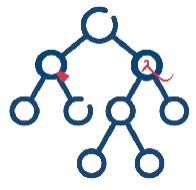
\includegraphics[height=1.0cm]{msca_logo.png}}%
    \end{center}

    \vspace{0.6cm}

    % Main title with Q logos on sides (with clickable links)
    \begin{center}
        \begin{minipage}{0.1\textwidth}
            \centering
            \href{https://quantlet.com}{
\includegraphics[height=1.1cm]{ql_logo.png}}
        \end{minipage}%
        \begin{minipage}{0.78\textwidth}
            \centering
            {\LARGE\bfseries\usebeamercolor[fg]{title}\inserttitle}

            \vspace{0.3cm}

            {\usebeamerfont{subtitle}\usebeamercolor[fg]{title}\insertsubtitle}
        \end{minipage}%
        \begin{minipage}{0.1\textwidth}
            \centering
            \href{https://quantinar.com}{
\includegraphics[height=1.1cm]{qr_logo.png}}
        \end{minipage}
    \end{center}

    \vspace{0.6cm}

    % Authors (left aligned)
    \hspace{0.5cm}{\usebeamerfont{author}\insertauthor}

    \vspace{0.3cm}

    % Institute/Affiliations (left aligned)
    \hspace{0.5cm}\begin{minipage}[t]{0.9\textwidth}
        \raggedright\small\insertinstitute
    \end{minipage}
}

%=============================================================================
% THEOREM ENVIRONMENTS
%=============================================================================
\theoremstyle{definition}
\setbeamertemplate{theorems}[numbered]
\ifdefined\tsalang
\newtheorem{defn}{Definiție}
\newtheorem{thm}{Teoremă}
\newtheorem{prop}{Propoziție}
\newtheorem{rmk}{Observație}
\else
\newtheorem{defn}{Definition}
\newtheorem{thm}{Theorem}
\newtheorem{prop}{Proposition}
\newtheorem{rmk}{Remark}
\fi

%=============================================================================
% CENTRED MINIPAGE (no extra vertical space)
%=============================================================================
\newenvironment{cminipage}[1]{%
    \par\noindent\hfill\begin{minipage}{#1}\ignorespaces
}{%
    \end{minipage}\hfill\null\par
}

%=============================================================================
% CUSTOM COMMANDS
%=============================================================================
\newcommand{\E}{\mathbb{E}}
\newcommand{\Var}{\text{Var}}
\newcommand{\Cov}{\text{Cov}}
\newcommand{\Corr}{\text{Corr}}
\newcommand{\R}{\mathbb{R}}
\newcommand{\N}{\mathbb{N}}
\newcommand{\Z}{\mathbb{Z}}
\newcommand{\B}{\mathbf{B}}
\newcommand{\imark}{\textcolor{MainBlue}{\textbullet}}
\newcommand{\RMSE}{\text{RMSE}}
\newcommand{\MAE}{\text{MAE}}
\newcommand{\MAPE}{\text{MAPE}}

% Boldface vector/matrix commands (VAR, VECM, state space; also used by the older TSA decks)
\newcommand{\bY}{\mathbf{Y}}
\newcommand{\bX}{\mathbf{X}}
\newcommand{\bA}{\mathbf{A}}
\newcommand{\bB}{\mathbf{B}}
\newcommand{\bepsilon}{\boldsymbol{\varepsilon}}
\newcommand{\bSigma}{\boldsymbol{\Sigma}}
\newcommand{\bPhi}{\boldsymbol{\Phi}}
\newcommand{\bGamma}{\boldsymbol{\Gamma}}
\newcommand{\bPi}{\boldsymbol{\Pi}}
\newcommand{\bc}{\mathbf{c}}
\newcommand{\balpha}{\boldsymbol{\alpha}}
\newcommand{\bbeta}{\boldsymbol{\beta}}
\newcommand{\bvarepsilon}{\boldsymbol{\varepsilon}}

% Legacy seminar marks (older TSA seminar decks)
\newcommand{\correct}{\textcolor{Forest}{\checkmark}}
\newcommand{\incorrect}{\textcolor{Crimson}{\texttimes}}
 se definește
%   \newcommand{\coursename}{Time Series Analysis}      (EN)
%   \newcommand{\coursename}{Serii de timp}       (RO)  și  \def\tsalang{ro}
% Fișierele .tex se află în EN/Courses, EN/Seminars, RO/Cursuri, RO/Seminarii (două niveluri sub rădăcină).
% Deck-urile sînt generate de latex/build_chapterN.py / build_seminarN.py (vezi latex/tsa_build.py).

\documentclass[9pt, aspectratio=169, t]{beamer}
\providecommand{\coursename}{Time Series Analysis}

% Ensure content fits on slides
\setbeamersize{text margin left=8mm, text margin right=8mm}
% Smaller institute font (title page)
\setbeamerfont{institute}{size=\footnotesize}

%=============================================================================
% THEME AND STYLE CONFIGURATION
%=============================================================================
\usetheme{default}
% Using default theme for clean header/footer control

% Color Palette (matching Redispatch PDF)
\definecolor{MainBlue}{RGB}{26, 58, 110}
\definecolor{AccentBlue}{RGB}{26, 58, 110}
\definecolor{IDAred}{RGB}{205, 0, 0}
\definecolor{DarkGray}{RGB}{51, 51, 51}
\definecolor{MediumGray}{RGB}{128, 128, 128}
\definecolor{LightGray}{RGB}{248, 248, 248}
\definecolor{VeryLightGray}{RGB}{235, 235, 235}
\definecolor{KeynoteGray}{RGB}{218, 218, 218}
\definecolor{SectionGray}{RGB}{120, 120, 120}
\definecolor{FooterGray}{RGB}{100, 100, 100}
\definecolor{Crimson}{RGB}{220, 53, 69}
\definecolor{Forest}{RGB}{46, 125, 50}
\definecolor{Amber}{RGB}{181, 133, 63}
\definecolor{Orange}{RGB}{230, 126, 34}
\definecolor{Purple}{RGB}{142, 68, 173}

% Gradient background (exact Keynote 315° gradient: white to RGB 218,218,218)
\setbeamertemplate{background}{%
    \begin{tikzpicture}[remember picture, overlay]
        \shade[shading=axis, shading angle=315,
        top color=white, bottom color=KeynoteGray]
        (current page.south west) rectangle (current page.north east);
    \end{tikzpicture}%
}
% Fallback solid color for compatibility
\setbeamercolor{background canvas}{bg=}

\setbeamercolor{palette primary}{bg=MainBlue, fg=white}
\setbeamercolor{palette secondary}{bg=MainBlue!85, fg=white}
\setbeamercolor{palette tertiary}{bg=MainBlue!70, fg=white}
\setbeamercolor{structure}{fg=MainBlue}
\setbeamercolor{title}{fg=IDAred}
\setbeamercolor{frametitle}{fg=IDAred, bg=}
\setbeamercolor{block title}{bg=MainBlue, fg=white}
\setbeamercolor{block body}{bg=VeryLightGray, fg=DarkGray}
\setbeamercolor{block title alerted}{bg=Crimson, fg=white}
\setbeamercolor{block body alerted}{bg=Crimson!8, fg=DarkGray}
\setbeamercolor{block title example}{bg=Forest, fg=white}
\setbeamercolor{block body example}{bg=Forest!8, fg=DarkGray}
\setbeamercolor{item}{fg=MainBlue}

% Footer colors (override Madrid theme blue)
\setbeamercolor{author in head/foot}{fg=FooterGray, bg=}
\setbeamercolor{title in head/foot}{fg=FooterGray, bg=}
\setbeamercolor{date in head/foot}{fg=FooterGray, bg=}
\setbeamercolor{section in head/foot}{fg=FooterGray, bg=}
\setbeamercolor{subsection in head/foot}{fg=FooterGray, bg=}

% Bullet styles (apply everywhere including blocks)
\setbeamertemplate{itemize item}{\color{MainBlue}$\boxdot$}
\setbeamertemplate{itemize subitem}{\color{MainBlue}$\blacktriangleright$}
\setbeamertemplate{itemize subsubitem}{\color{MainBlue}\tiny$\bullet$}
\setbeamertemplate{itemize/enumerate body begin}{\normalsize}
\setbeamertemplate{itemize/enumerate subbody begin}{\normalsize}

% Item spacing - compact style
\setlength{\leftmargini}{10pt}       % Level 1: minimal indent
\setlength{\leftmarginii}{10pt}      % Level 2: minimal additional indent
% Compact list spacing (zero extra space before/after lists in blocks)
\makeatletter
\def\@listi{\leftmargin\leftmargini \topsep 0pt \parsep 0pt \itemsep 0pt}
\def\@listii{\leftmargin\leftmarginii \topsep 0pt \parsep 0pt \itemsep 0pt}
\makeatother

\setbeamertemplate{navigation symbols}{}

%=============================================================================
% CUSTOM HEADLINE
%=============================================================================
\setbeamertemplate{headline}{%
    \vskip10pt%
    \hbox to \paperwidth{%
        \hskip0.5cm%
        {\small\color{FooterGray}\renewcommand{\hyperlink}[2]{##2}\insertsectionhead}%
        \hfill%
        \textcolor{FooterGray}{\small\insertframenumber}%
        \hskip0.5cm%
    }%
    \vskip4pt%
    {\color{FooterGray}\hrule height 0.4pt}%
}

%=============================================================================
% CUSTOM FOOTER
%=============================================================================
\usepackage{fontawesome5}

\setbeamertemplate{footline}{%
    {\color{FooterGray}\hrule height 0.4pt}%
    \vskip4pt%
    \hbox to \paperwidth{%
        \hskip0.5cm%
        \textcolor{FooterGray}{\small\coursename}%
        \hfill%
        \raisebox{-0.1em}{%
            \begin{tikzpicture}[x=0.08em, y=0.08em, line width=0.4pt]
                \draw[FooterGray] (0,3) -- (1,4) -- (2,3.5) -- (3,5) -- (4,4) -- (5,6) -- (6,5.5) -- (7,4) -- (8,5) -- (9,7) -- (10,6) -- (11,5) -- (12,6.5) -- (13,8) -- (14,7) -- (15,6) -- (16,7.5) -- (17,9) -- (18,8) -- (19,7) -- (20,8.5) -- (21,10) -- (22,9) -- (23,8) -- (24,9.5);
            \end{tikzpicture}%
        }%
        \hskip0.5cm%
    }%
    \vskip6pt%
}

%=============================================================================
% PACKAGES
%=============================================================================
\usepackage[utf8]{inputenc}
\DeclareUnicodeCharacter{03B1}{\ensuremath{\alpha}}
\usepackage[T1]{fontenc}
\usepackage{amsmath, amssymb, amsthm}
\usepackage{mathtools}
\usepackage{bm}
\usepackage{tikz}
\usetikzlibrary{arrows.meta, positioning, shapes, calc, decorations.pathreplacing, shadings}
\usepackage{booktabs}
\usepackage{multirow}
\usepackage{array}
\usepackage{graphicx}
\usepackage{animate}
\usepackage{hyperref}
\usepackage{colortbl}
\usepackage{listings}
\lstset{language=Python, basicstyle=\ttfamily\scriptsize, keywordstyle=\color{MainBlue}\bfseries,
  commentstyle=\color{Forest}, stringstyle=\color{Crimson}, breaklines=true,
  frame=none, backgroundcolor=\color{VeryLightGray}, xleftmargin=2mm}
\hypersetup{colorlinks=true, linkcolor=MainBlue, urlcolor=MainBlue}
\graphicspath{{../../logos/}{../../charts/}{../../photos/}}
\usepackage{xcolor}
\hfuzz=2pt  % Suppress tiny overfull warnings (<2pt)
\vfuzz=2pt  % Suppress tiny vertical overfull warnings (<2pt)
% \mathrm in the sans-serif family of the slides (beamer resets \mathrm to the serif family at \begin{document};
% this hook runs after beamer's, so WN, Var, RMSE, ... in formulas match the surrounding text)
% Bold vectors and matrices in the same sans-serif family: \mathbf{A} in sans bold (beamer's own \mathbf came out in
% medium weight), and the bold upright Greek capitals of \boldsymbol / \bm (\bSigma, \bPhi, \boldsymbol{\Theta}) in
% cmss bold: bm.sty fixes its "boldoperators" font when it is loaded (serif cmbx), before beamer switches the
% operators to cmss, so it is reset here.
\AtBeginDocument{%
  \SetMathAlphabet{\mathrm}{normal}{\encodingdefault}{\sfdefault}{\mddefault}{n}%
  \SetMathAlphabet{\mathrm}{bold}{\encodingdefault}{\sfdefault}{bx}{n}%
  \SetMathAlphabet{\mathbf}{normal}{\encodingdefault}{\sfdefault}{bx}{n}%
  \SetMathAlphabet{\mathbf}{bold}{\encodingdefault}{\sfdefault}{bx}{n}%
  \SetSymbolFont{boldoperators}{normal}{OT1}{cmss}{bx}{n}%
  \SetSymbolFont{boldoperators}{bold}{OT1}{cmss}{bx}{n}}

%=============================================================================
% QUANTLET COMMANDS
%   \quantlet{<displayed name>}{<url>}       (generic, compatible with the older TSA decks)
%   \tsaquantlet{Ch_05}{TSA_ch5_garch}       -> https://github.com/danpele/Time-Series-Analysis/tree/main/Quantlets/Ch_05/TSA_ch5_garch
%   \qlurl{<folder>} is defined per chapter by the generator (Quantlets/Ch_NN/<folder>)
%=============================================================================
\newcommand{\tsarepo}{https://github.com/danpele/Time-Series-Analysis}
\newcommand{\tsaqlbase}{https://github.com/danpele/Time-Series-Analysis/tree/main/Quantlets}
\newcommand{\quantlet}[2]{%
    \hfill\href{#2}{%
        \raisebox{-0.15em}{
\includegraphics[height=0.7em]{ql_logo.png}}%
        \textcolor{MainBlue}{\tiny\ #1}%
    }%
}
\newcommand{\tsaquantlet}[2]{\quantlet{\detokenize{#2}}{\tsaqlbase/#1/#2}}

%=============================================================================
% NOTEBOOKS (Google Colab)
%   \colaburl{notebooks/EN/chapter5_seminar_notebook.ipynb} -> the Colab link of a file in the TSA repo
%   \nb: the chapter notebook (each seminar deck redefines it with \renewcommand)
%=============================================================================
\newcommand{\colaburl}[1]{https://colab.research.google.com/github/danpele/Time-Series-Analysis/blob/main/#1}
\newcommand{\nb}{https://colab.research.google.com/github/danpele/Time-Series-Analysis/tree/main/notebooks/EN}
\newcommand{\nbname}{notebooks/EN}

%=============================================================================
% SLIDE HELPERS (used by the generators; the same as in MFM)
%=============================================================================
% local font size for list bodies (the preamble forces \normalsize)
\newcommand{\itemsize}[1]{\setbeamertemplate{itemize/enumerate body begin}{#1}\setbeamertemplate{itemize/enumerate subbody begin}{#1}}
\newcommand{\intitle}[1]{{\hypersetup{urlcolor=white}#1}}   % white links inside coloured title bars
\newcommand{\imgcap}[1]{{\scriptsize #1}\\[0.5mm]}          % caption under a photo
\newcommand{\imgcredit}[2]{{\tiny\color{FooterGray}\href{#1}{#2}}}   % image credit: source URL, author/licence
\newcommand{\aiprompt}[1]{{\ttfamily\color{MainBlue}#1}}     % a prompt to an AI assistant

%=============================================================================
% SEMINARS: student version by default; the instructor wrapper *_solutions.tex sets \solutionstrue
%=============================================================================
\makeatletter\@ifundefined{ifsolutions}{\expandafter\newif\csname ifsolutions\endcsname}{}\makeatother
\newcommand{\solonly}[1]{\ifsolutions #1\fi}
\newcommand{\propsub}{\ifsolutions\else\framesubtitle{\ifdefined\tsalang Rezolvarea se discută la seminar\else Solution discussed in class\fi}\fi}

%=============================================================================
% APPENDIX AND CHAPTER LINKS (latex/appendix_links.py writes the calls; it also re-declares these
% macros before \begin{document}, so the decks compile with or without this preamble block)
%=============================================================================
\providecommand{\tsaapplink}[3]{\hypertarget{#2}{}\hyperlink{#1}{\beamergotobutton{#3}}}
\providecommand{\tsaappback}[2]{\begin{tikzpicture}[remember picture,overlay]\node[anchor=south east] at ([xshift=-3mm,yshift=7mm]current page.south east){\hyperlink{#1}{\beamerreturnbutton{#2}}};\end{tikzpicture}}
\providecommand{\tsachlink}[2]{\href{#1}{#2}}
\providecommand{\tsachlinkt}[2]{\href{#1}{\usebeamercolor[fg]{frametitle}#2}}

%=============================================================================
% QUANTINAR COMMAND: link către un curs Quantinar (subiecte avansate)
%=============================================================================
\newcommand{\quantinar}[2]{%
    \href{#2}{%
        \raisebox{-0.15em}{
\includegraphics[height=0.8em]{qr_logo.png}}%
        \textcolor{MainBlue}{\scriptsize\ #1}%
    }%
}

%=============================================================================
% CUSTOM TITLE PAGE
%=============================================================================
\defbeamertemplate*{title page}{hybrid}[1][]
{
    \vspace{0.2cm}
    % Logos row - top header (with clickable links)
    \begin{center}
        \href{https://www.ase.ro}{
\includegraphics[height=1.0cm]{ase_logo.png}}\hspace{0.3cm}%
        \href{https://theida.net}{
\includegraphics[height=1.0cm]{ida_logo.png}}\hspace{0.3cm}%
        \href{https://blockchain-research-center.com}{
\includegraphics[height=1.0cm]{brc_logo.png}}\hspace{0.3cm}%
        \href{https://www.ai4efin.ase.ro}{
\includegraphics[height=1.0cm]{ai4efin_logo.png}}\hspace{0.3cm}%
        \href{https://ipe.ro/new}{
\includegraphics[height=1.0cm]{acad_logo.png}}\hspace{0.3cm}%
        \href{https://www.digital-finance-msca.com}{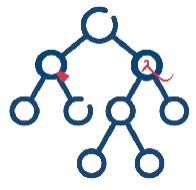
\includegraphics[height=1.0cm]{msca_logo.png}}%
    \end{center}

    \vspace{0.6cm}

    % Main title with Q logos on sides (with clickable links)
    \begin{center}
        \begin{minipage}{0.1\textwidth}
            \centering
            \href{https://quantlet.com}{
\includegraphics[height=1.1cm]{ql_logo.png}}
        \end{minipage}%
        \begin{minipage}{0.78\textwidth}
            \centering
            {\LARGE\bfseries\usebeamercolor[fg]{title}\inserttitle}

            \vspace{0.3cm}

            {\usebeamerfont{subtitle}\usebeamercolor[fg]{title}\insertsubtitle}
        \end{minipage}%
        \begin{minipage}{0.1\textwidth}
            \centering
            \href{https://quantinar.com}{
\includegraphics[height=1.1cm]{qr_logo.png}}
        \end{minipage}
    \end{center}

    \vspace{0.6cm}

    % Authors (left aligned)
    \hspace{0.5cm}{\usebeamerfont{author}\insertauthor}

    \vspace{0.3cm}

    % Institute/Affiliations (left aligned)
    \hspace{0.5cm}\begin{minipage}[t]{0.9\textwidth}
        \raggedright\small\insertinstitute
    \end{minipage}
}

%=============================================================================
% THEOREM ENVIRONMENTS
%=============================================================================
\theoremstyle{definition}
\setbeamertemplate{theorems}[numbered]
\ifdefined\tsalang
\newtheorem{defn}{Definiție}
\newtheorem{thm}{Teoremă}
\newtheorem{prop}{Propoziție}
\newtheorem{rmk}{Observație}
\else
\newtheorem{defn}{Definition}
\newtheorem{thm}{Theorem}
\newtheorem{prop}{Proposition}
\newtheorem{rmk}{Remark}
\fi

%=============================================================================
% CENTRED MINIPAGE (no extra vertical space)
%=============================================================================
\newenvironment{cminipage}[1]{%
    \par\noindent\hfill\begin{minipage}{#1}\ignorespaces
}{%
    \end{minipage}\hfill\null\par
}

%=============================================================================
% CUSTOM COMMANDS
%=============================================================================
\newcommand{\E}{\mathbb{E}}
\newcommand{\Var}{\text{Var}}
\newcommand{\Cov}{\text{Cov}}
\newcommand{\Corr}{\text{Corr}}
\newcommand{\R}{\mathbb{R}}
\newcommand{\N}{\mathbb{N}}
\newcommand{\Z}{\mathbb{Z}}
\newcommand{\B}{\mathbf{B}}
\newcommand{\imark}{\textcolor{MainBlue}{\textbullet}}
\newcommand{\RMSE}{\text{RMSE}}
\newcommand{\MAE}{\text{MAE}}
\newcommand{\MAPE}{\text{MAPE}}

% Boldface vector/matrix commands (VAR, VECM, state space; also used by the older TSA decks)
\newcommand{\bY}{\mathbf{Y}}
\newcommand{\bX}{\mathbf{X}}
\newcommand{\bA}{\mathbf{A}}
\newcommand{\bB}{\mathbf{B}}
\newcommand{\bepsilon}{\boldsymbol{\varepsilon}}
\newcommand{\bSigma}{\boldsymbol{\Sigma}}
\newcommand{\bPhi}{\boldsymbol{\Phi}}
\newcommand{\bGamma}{\boldsymbol{\Gamma}}
\newcommand{\bPi}{\boldsymbol{\Pi}}
\newcommand{\bc}{\mathbf{c}}
\newcommand{\balpha}{\boldsymbol{\alpha}}
\newcommand{\bbeta}{\boldsymbol{\beta}}
\newcommand{\bvarepsilon}{\boldsymbol{\varepsilon}}

% Legacy seminar marks (older TSA seminar decks)
\newcommand{\correct}{\textcolor{Forest}{\checkmark}}
\newcommand{\incorrect}{\textcolor{Crimson}{\texttimes}}
 se definește
%   \newcommand{\coursename}{Time Series Analysis}      (EN)
%   \newcommand{\coursename}{Serii de timp}       (RO)  și  \def\tsalang{ro}
% Fișierele .tex se află în EN/Courses, EN/Seminars, RO/Cursuri, RO/Seminarii (două niveluri sub rădăcină).
% Deck-urile sînt generate de latex/build_chapterN.py / build_seminarN.py (vezi latex/tsa_build.py).

\documentclass[9pt, aspectratio=169, t]{beamer}
\providecommand{\coursename}{Time Series Analysis}

% Ensure content fits on slides
\setbeamersize{text margin left=8mm, text margin right=8mm}
% Smaller institute font (title page)
\setbeamerfont{institute}{size=\footnotesize}

%=============================================================================
% THEME AND STYLE CONFIGURATION
%=============================================================================
\usetheme{default}
% Using default theme for clean header/footer control

% Color Palette (matching Redispatch PDF)
\definecolor{MainBlue}{RGB}{26, 58, 110}
\definecolor{AccentBlue}{RGB}{26, 58, 110}
\definecolor{IDAred}{RGB}{205, 0, 0}
\definecolor{DarkGray}{RGB}{51, 51, 51}
\definecolor{MediumGray}{RGB}{128, 128, 128}
\definecolor{LightGray}{RGB}{248, 248, 248}
\definecolor{VeryLightGray}{RGB}{235, 235, 235}
\definecolor{KeynoteGray}{RGB}{218, 218, 218}
\definecolor{SectionGray}{RGB}{120, 120, 120}
\definecolor{FooterGray}{RGB}{100, 100, 100}
\definecolor{Crimson}{RGB}{220, 53, 69}
\definecolor{Forest}{RGB}{46, 125, 50}
\definecolor{Amber}{RGB}{181, 133, 63}
\definecolor{Orange}{RGB}{230, 126, 34}
\definecolor{Purple}{RGB}{142, 68, 173}

% Gradient background (exact Keynote 315° gradient: white to RGB 218,218,218)
\setbeamertemplate{background}{%
    \begin{tikzpicture}[remember picture, overlay]
        \shade[shading=axis, shading angle=315,
        top color=white, bottom color=KeynoteGray]
        (current page.south west) rectangle (current page.north east);
    \end{tikzpicture}%
}
% Fallback solid color for compatibility
\setbeamercolor{background canvas}{bg=}

\setbeamercolor{palette primary}{bg=MainBlue, fg=white}
\setbeamercolor{palette secondary}{bg=MainBlue!85, fg=white}
\setbeamercolor{palette tertiary}{bg=MainBlue!70, fg=white}
\setbeamercolor{structure}{fg=MainBlue}
\setbeamercolor{title}{fg=IDAred}
\setbeamercolor{frametitle}{fg=IDAred, bg=}
\setbeamercolor{block title}{bg=MainBlue, fg=white}
\setbeamercolor{block body}{bg=VeryLightGray, fg=DarkGray}
\setbeamercolor{block title alerted}{bg=Crimson, fg=white}
\setbeamercolor{block body alerted}{bg=Crimson!8, fg=DarkGray}
\setbeamercolor{block title example}{bg=Forest, fg=white}
\setbeamercolor{block body example}{bg=Forest!8, fg=DarkGray}
\setbeamercolor{item}{fg=MainBlue}

% Footer colors (override Madrid theme blue)
\setbeamercolor{author in head/foot}{fg=FooterGray, bg=}
\setbeamercolor{title in head/foot}{fg=FooterGray, bg=}
\setbeamercolor{date in head/foot}{fg=FooterGray, bg=}
\setbeamercolor{section in head/foot}{fg=FooterGray, bg=}
\setbeamercolor{subsection in head/foot}{fg=FooterGray, bg=}

% Bullet styles (apply everywhere including blocks)
\setbeamertemplate{itemize item}{\color{MainBlue}$\boxdot$}
\setbeamertemplate{itemize subitem}{\color{MainBlue}$\blacktriangleright$}
\setbeamertemplate{itemize subsubitem}{\color{MainBlue}\tiny$\bullet$}
\setbeamertemplate{itemize/enumerate body begin}{\normalsize}
\setbeamertemplate{itemize/enumerate subbody begin}{\normalsize}

% Item spacing - compact style
\setlength{\leftmargini}{10pt}       % Level 1: minimal indent
\setlength{\leftmarginii}{10pt}      % Level 2: minimal additional indent
% Compact list spacing (zero extra space before/after lists in blocks)
\makeatletter
\def\@listi{\leftmargin\leftmargini \topsep 0pt \parsep 0pt \itemsep 0pt}
\def\@listii{\leftmargin\leftmarginii \topsep 0pt \parsep 0pt \itemsep 0pt}
\makeatother

\setbeamertemplate{navigation symbols}{}

%=============================================================================
% CUSTOM HEADLINE
%=============================================================================
\setbeamertemplate{headline}{%
    \vskip10pt%
    \hbox to \paperwidth{%
        \hskip0.5cm%
        {\small\color{FooterGray}\renewcommand{\hyperlink}[2]{##2}\insertsectionhead}%
        \hfill%
        \textcolor{FooterGray}{\small\insertframenumber}%
        \hskip0.5cm%
    }%
    \vskip4pt%
    {\color{FooterGray}\hrule height 0.4pt}%
}

%=============================================================================
% CUSTOM FOOTER
%=============================================================================
\usepackage{fontawesome5}

\setbeamertemplate{footline}{%
    {\color{FooterGray}\hrule height 0.4pt}%
    \vskip4pt%
    \hbox to \paperwidth{%
        \hskip0.5cm%
        \textcolor{FooterGray}{\small\coursename}%
        \hfill%
        \raisebox{-0.1em}{%
            \begin{tikzpicture}[x=0.08em, y=0.08em, line width=0.4pt]
                \draw[FooterGray] (0,3) -- (1,4) -- (2,3.5) -- (3,5) -- (4,4) -- (5,6) -- (6,5.5) -- (7,4) -- (8,5) -- (9,7) -- (10,6) -- (11,5) -- (12,6.5) -- (13,8) -- (14,7) -- (15,6) -- (16,7.5) -- (17,9) -- (18,8) -- (19,7) -- (20,8.5) -- (21,10) -- (22,9) -- (23,8) -- (24,9.5);
            \end{tikzpicture}%
        }%
        \hskip0.5cm%
    }%
    \vskip6pt%
}

%=============================================================================
% PACKAGES
%=============================================================================
\usepackage[utf8]{inputenc}
\DeclareUnicodeCharacter{03B1}{\ensuremath{\alpha}}
\usepackage[T1]{fontenc}
\usepackage{amsmath, amssymb, amsthm}
\usepackage{mathtools}
\usepackage{bm}
\usepackage{tikz}
\usetikzlibrary{arrows.meta, positioning, shapes, calc, decorations.pathreplacing, shadings}
\usepackage{booktabs}
\usepackage{multirow}
\usepackage{array}
\usepackage{graphicx}
\usepackage{animate}
\usepackage{hyperref}
\usepackage{colortbl}
\usepackage{listings}
\lstset{language=Python, basicstyle=\ttfamily\scriptsize, keywordstyle=\color{MainBlue}\bfseries,
  commentstyle=\color{Forest}, stringstyle=\color{Crimson}, breaklines=true,
  frame=none, backgroundcolor=\color{VeryLightGray}, xleftmargin=2mm}
\hypersetup{colorlinks=true, linkcolor=MainBlue, urlcolor=MainBlue}
\graphicspath{{../../logos/}{../../charts/}{../../photos/}}
\usepackage{xcolor}
\hfuzz=2pt  % Suppress tiny overfull warnings (<2pt)
\vfuzz=2pt  % Suppress tiny vertical overfull warnings (<2pt)
% \mathrm in the sans-serif family of the slides (beamer resets \mathrm to the serif family at \begin{document};
% this hook runs after beamer's, so WN, Var, RMSE, ... in formulas match the surrounding text)
% Bold vectors and matrices in the same sans-serif family: \mathbf{A} in sans bold (beamer's own \mathbf came out in
% medium weight), and the bold upright Greek capitals of \boldsymbol / \bm (\bSigma, \bPhi, \boldsymbol{\Theta}) in
% cmss bold: bm.sty fixes its "boldoperators" font when it is loaded (serif cmbx), before beamer switches the
% operators to cmss, so it is reset here.
\AtBeginDocument{%
  \SetMathAlphabet{\mathrm}{normal}{\encodingdefault}{\sfdefault}{\mddefault}{n}%
  \SetMathAlphabet{\mathrm}{bold}{\encodingdefault}{\sfdefault}{bx}{n}%
  \SetMathAlphabet{\mathbf}{normal}{\encodingdefault}{\sfdefault}{bx}{n}%
  \SetMathAlphabet{\mathbf}{bold}{\encodingdefault}{\sfdefault}{bx}{n}%
  \SetSymbolFont{boldoperators}{normal}{OT1}{cmss}{bx}{n}%
  \SetSymbolFont{boldoperators}{bold}{OT1}{cmss}{bx}{n}}

%=============================================================================
% QUANTLET COMMANDS
%   \quantlet{<displayed name>}{<url>}       (generic, compatible with the older TSA decks)
%   \tsaquantlet{Ch_05}{TSA_ch5_garch}       -> https://github.com/danpele/Time-Series-Analysis/tree/main/Quantlets/Ch_05/TSA_ch5_garch
%   \qlurl{<folder>} is defined per chapter by the generator (Quantlets/Ch_NN/<folder>)
%=============================================================================
\newcommand{\tsarepo}{https://github.com/danpele/Time-Series-Analysis}
\newcommand{\tsaqlbase}{https://github.com/danpele/Time-Series-Analysis/tree/main/Quantlets}
\newcommand{\quantlet}[2]{%
    \hfill\href{#2}{%
        \raisebox{-0.15em}{
\includegraphics[height=0.7em]{ql_logo.png}}%
        \textcolor{MainBlue}{\tiny\ #1}%
    }%
}
\newcommand{\tsaquantlet}[2]{\quantlet{\detokenize{#2}}{\tsaqlbase/#1/#2}}

%=============================================================================
% NOTEBOOKS (Google Colab)
%   \colaburl{notebooks/EN/chapter5_seminar_notebook.ipynb} -> the Colab link of a file in the TSA repo
%   \nb: the chapter notebook (each seminar deck redefines it with \renewcommand)
%=============================================================================
\newcommand{\colaburl}[1]{https://colab.research.google.com/github/danpele/Time-Series-Analysis/blob/main/#1}
\newcommand{\nb}{https://colab.research.google.com/github/danpele/Time-Series-Analysis/tree/main/notebooks/EN}
\newcommand{\nbname}{notebooks/EN}

%=============================================================================
% SLIDE HELPERS (used by the generators; the same as in MFM)
%=============================================================================
% local font size for list bodies (the preamble forces \normalsize)
\newcommand{\itemsize}[1]{\setbeamertemplate{itemize/enumerate body begin}{#1}\setbeamertemplate{itemize/enumerate subbody begin}{#1}}
\newcommand{\intitle}[1]{{\hypersetup{urlcolor=white}#1}}   % white links inside coloured title bars
\newcommand{\imgcap}[1]{{\scriptsize #1}\\[0.5mm]}          % caption under a photo
\newcommand{\imgcredit}[2]{{\tiny\color{FooterGray}\href{#1}{#2}}}   % image credit: source URL, author/licence
\newcommand{\aiprompt}[1]{{\ttfamily\color{MainBlue}#1}}     % a prompt to an AI assistant

%=============================================================================
% SEMINARS: student version by default; the instructor wrapper *_solutions.tex sets \solutionstrue
%=============================================================================
\makeatletter\@ifundefined{ifsolutions}{\expandafter\newif\csname ifsolutions\endcsname}{}\makeatother
\newcommand{\solonly}[1]{\ifsolutions #1\fi}
\newcommand{\propsub}{\ifsolutions\else\framesubtitle{\ifdefined\tsalang Rezolvarea se discută la seminar\else Solution discussed in class\fi}\fi}

%=============================================================================
% APPENDIX AND CHAPTER LINKS (latex/appendix_links.py writes the calls; it also re-declares these
% macros before \begin{document}, so the decks compile with or without this preamble block)
%=============================================================================
\providecommand{\tsaapplink}[3]{\hypertarget{#2}{}\hyperlink{#1}{\beamergotobutton{#3}}}
\providecommand{\tsaappback}[2]{\begin{tikzpicture}[remember picture,overlay]\node[anchor=south east] at ([xshift=-3mm,yshift=7mm]current page.south east){\hyperlink{#1}{\beamerreturnbutton{#2}}};\end{tikzpicture}}
\providecommand{\tsachlink}[2]{\href{#1}{#2}}
\providecommand{\tsachlinkt}[2]{\href{#1}{\usebeamercolor[fg]{frametitle}#2}}

%=============================================================================
% QUANTINAR COMMAND: link către un curs Quantinar (subiecte avansate)
%=============================================================================
\newcommand{\quantinar}[2]{%
    \href{#2}{%
        \raisebox{-0.15em}{
\includegraphics[height=0.8em]{qr_logo.png}}%
        \textcolor{MainBlue}{\scriptsize\ #1}%
    }%
}

%=============================================================================
% CUSTOM TITLE PAGE
%=============================================================================
\defbeamertemplate*{title page}{hybrid}[1][]
{
    \vspace{0.2cm}
    % Logos row - top header (with clickable links)
    \begin{center}
        \href{https://www.ase.ro}{
\includegraphics[height=1.0cm]{ase_logo.png}}\hspace{0.3cm}%
        \href{https://theida.net}{
\includegraphics[height=1.0cm]{ida_logo.png}}\hspace{0.3cm}%
        \href{https://blockchain-research-center.com}{
\includegraphics[height=1.0cm]{brc_logo.png}}\hspace{0.3cm}%
        \href{https://www.ai4efin.ase.ro}{
\includegraphics[height=1.0cm]{ai4efin_logo.png}}\hspace{0.3cm}%
        \href{https://ipe.ro/new}{
\includegraphics[height=1.0cm]{acad_logo.png}}\hspace{0.3cm}%
        \href{https://www.digital-finance-msca.com}{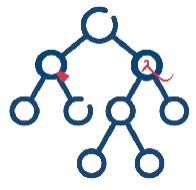
\includegraphics[height=1.0cm]{msca_logo.png}}%
    \end{center}

    \vspace{0.6cm}

    % Main title with Q logos on sides (with clickable links)
    \begin{center}
        \begin{minipage}{0.1\textwidth}
            \centering
            \href{https://quantlet.com}{
\includegraphics[height=1.1cm]{ql_logo.png}}
        \end{minipage}%
        \begin{minipage}{0.78\textwidth}
            \centering
            {\LARGE\bfseries\usebeamercolor[fg]{title}\inserttitle}

            \vspace{0.3cm}

            {\usebeamerfont{subtitle}\usebeamercolor[fg]{title}\insertsubtitle}
        \end{minipage}%
        \begin{minipage}{0.1\textwidth}
            \centering
            \href{https://quantinar.com}{
\includegraphics[height=1.1cm]{qr_logo.png}}
        \end{minipage}
    \end{center}

    \vspace{0.6cm}

    % Authors (left aligned)
    \hspace{0.5cm}{\usebeamerfont{author}\insertauthor}

    \vspace{0.3cm}

    % Institute/Affiliations (left aligned)
    \hspace{0.5cm}\begin{minipage}[t]{0.9\textwidth}
        \raggedright\small\insertinstitute
    \end{minipage}
}

%=============================================================================
% THEOREM ENVIRONMENTS
%=============================================================================
\theoremstyle{definition}
\setbeamertemplate{theorems}[numbered]
\ifdefined\tsalang
\newtheorem{defn}{Definiție}
\newtheorem{thm}{Teoremă}
\newtheorem{prop}{Propoziție}
\newtheorem{rmk}{Observație}
\else
\newtheorem{defn}{Definition}
\newtheorem{thm}{Theorem}
\newtheorem{prop}{Proposition}
\newtheorem{rmk}{Remark}
\fi

%=============================================================================
% CENTRED MINIPAGE (no extra vertical space)
%=============================================================================
\newenvironment{cminipage}[1]{%
    \par\noindent\hfill\begin{minipage}{#1}\ignorespaces
}{%
    \end{minipage}\hfill\null\par
}

%=============================================================================
% CUSTOM COMMANDS
%=============================================================================
\newcommand{\E}{\mathbb{E}}
\newcommand{\Var}{\text{Var}}
\newcommand{\Cov}{\text{Cov}}
\newcommand{\Corr}{\text{Corr}}
\newcommand{\R}{\mathbb{R}}
\newcommand{\N}{\mathbb{N}}
\newcommand{\Z}{\mathbb{Z}}
\newcommand{\B}{\mathbf{B}}
\newcommand{\imark}{\textcolor{MainBlue}{\textbullet}}
\newcommand{\RMSE}{\text{RMSE}}
\newcommand{\MAE}{\text{MAE}}
\newcommand{\MAPE}{\text{MAPE}}

% Boldface vector/matrix commands (VAR, VECM, state space; also used by the older TSA decks)
\newcommand{\bY}{\mathbf{Y}}
\newcommand{\bX}{\mathbf{X}}
\newcommand{\bA}{\mathbf{A}}
\newcommand{\bB}{\mathbf{B}}
\newcommand{\bepsilon}{\boldsymbol{\varepsilon}}
\newcommand{\bSigma}{\boldsymbol{\Sigma}}
\newcommand{\bPhi}{\boldsymbol{\Phi}}
\newcommand{\bGamma}{\boldsymbol{\Gamma}}
\newcommand{\bPi}{\boldsymbol{\Pi}}
\newcommand{\bc}{\mathbf{c}}
\newcommand{\balpha}{\boldsymbol{\alpha}}
\newcommand{\bbeta}{\boldsymbol{\beta}}
\newcommand{\bvarepsilon}{\boldsymbol{\varepsilon}}

% Legacy seminar marks (older TSA seminar decks)
\newcommand{\correct}{\textcolor{Forest}{\checkmark}}
\newcommand{\incorrect}{\textcolor{Crimson}{\texttimes}}


\newcommand{\qlurl}[1]{https://github.com/danpele/Time-Series-Analysis/tree/main/Quantlets/Ch_15/#1}
\renewcommand{\nb}{\colaburl{notebooks/EN/chapter15_seminar_notebook.ipynb}}
\renewcommand{\nbname}{chapter15\_seminar\_notebook.ipynb}
% left column: full width in the student version, narrower next to the solution
\newcommand{\taskw}{\ifsolutions 0.47\textwidth\else 0.96\textwidth\fi}
\newcommand{\solw}{\ifsolutions 0.49\textwidth\else 0pt\fi}

% Clickable citations (DOIs verified via Crossref)
\newcommand{\refHP}{\href{https://doi.org/10.1007/978-3-031-13584-2}{Huang și Petukhina (2022)}}
\newcommand{\refFPP}{\href{https://otexts.com/fpp3/}{Hyndman și Athanasopoulos (2021)}}
\newcommand{\refBD}{\href{https://doi.org/10.1007/978-3-319-29854-2}{Brockwell și Davis (2016)}}
\newcommand{\refHamilton}{\href{https://doi.org/10.2307/j.ctv14jx6sm}{Hamilton (1994)}}
\newcommand{\refBJ}{\href{https://doi.org/10.1002/9781118619193}{Box, Jenkins și Reinsel (2008)}}
\newcommand{\refLB}{\href{https://doi.org/10.1093/biomet/65.2.297}{Ljung și Box (1978)}}
\newcommand{\refAkaike}{\href{https://doi.org/10.1109/TAC.1974.1100705}{Akaike (1974)}}
\newcommand{\refSchwarz}{\href{https://doi.org/10.1214/aos/1176344136}{Schwarz (1978)}}
\newcommand{\refDF}{\href{https://doi.org/10.1080/01621459.1979.10482531}{Dickey și Fuller (1979)}}
\newcommand{\refKPSS}{\href{https://doi.org/10.1016/0304-4076(92)90104-Y}{Kwiatkowski et al.\ (1992)}}
\newcommand{\refGN}{\href{https://doi.org/10.1016/0304-4076(74)90034-7}{Granger și Newbold (1974)}}
\newcommand{\refDM}{\href{https://doi.org/10.1080/07350015.1995.10524599}{Diebold și Mariano (1995)}}
\newcommand{\refHLN}{\href{https://doi.org/10.1016/S0169-2070(96)00719-4}{Harvey, Leybourne și Newbold (1997)}}
\newcommand{\refEngle}{\href{https://doi.org/10.2307/1912773}{Engle (1982)}}
\newcommand{\refBoll}{\href{https://doi.org/10.1016/0304-4076(86)90063-1}{Bollerslev (1986)}}
\newcommand{\refSims}{\href{https://doi.org/10.2307/1912017}{Sims (1980)}}
\newcommand{\refGranger}{\href{https://doi.org/10.2307/1912791}{Granger (1969)}}
\newcommand{\refEG}{\href{https://doi.org/10.2307/1913236}{Engle și Granger (1987)}}
\newcommand{\refJoh}{\href{https://doi.org/10.2307/2938278}{Johansen (1991)}}
\newcommand{\refGJ}{\href{https://doi.org/10.1111/j.1467-9892.1980.tb00297.x}{Granger și Joyeux (1980)}}
\newcommand{\refHosking}{\href{https://doi.org/10.1093/biomet/68.1.165}{Hosking (1981)}}
\newcommand{\refMfour}{\href{https://doi.org/10.1016/j.ijforecast.2019.04.014}{Makridakis, Spiliotis și Assimakopoulos (2020)}}
\newcommand{\refKalman}{\href{https://doi.org/10.1115/1.3662552}{Kalman (1960)}}
\newcommand{\refHamMS}{\href{https://doi.org/10.2307/1912559}{Hamilton (1989)}}

\title[Serii de timp]{Serii de timp}
\subtitle{Seminarul 15: Recapitulare și pregătire pentru examen\ifsolutions\ (versiunea profesorului)\fi}
\author[D.T. Pele]{Daniel Traian PELE}
\institute{Academia de Studii Economice din București\\
IDA Institute Digital Assets\\
Blockchain Research Center\\
AI4EFin Artificial Intelligence for Energy Finance\\
Academia Română, Institutul de Prognoză Economică\\
MSCA Digital Finance}
\date{}

%=============================================================================
\providecommand{\tsaapplink}[3]{\hypertarget{#2}{}\hyperlink{#1}{\beamergotobutton{#3}}}  % APPLINKS-MACROS
\providecommand{\tsaappback}[2]{\begin{tikzpicture}[remember picture,overlay]\node[anchor=south east] at ([xshift=-3mm,yshift=7mm]current page.south east){\hyperlink{#1}{\beamerreturnbutton{#2}}};\end{tikzpicture}}  % APPLINKS-MACROS
\providecommand{\tsachlink}[2]{\href{#1}{#2}}  % APPLINKS-MACROS
\providecommand{\tsachlinkt}[2]{\href{#1}{\usebeamercolor[fg]{frametitle}#2}}  % APPLINKS-MACROS
\begin{document}
%=============================================================================

{
\setbeamertemplate{headline}{}
\setbeamertemplate{footline}{}
\begin{frame}[noframenumbering]
    \titlepage
\end{frame}
}
% BEGIN-ACRONYMS (generat de latex/acronyms.py; nu editati manual)
\begin{frame}{Acronime folosite în acest material (1/2)}
\setbeamertemplate{itemize/enumerate body begin}{\tiny}
\begin{columns}[T]
\begin{column}{0.49\textwidth}
\begin{itemize}\setlength{\itemsep}{0pt}
    \item \textbf{ACF}: Autocorrelation Function (funcția de autocorelație)
    \item \textbf{ADF}: Augmented Dickey–Fuller (test) — testul Dickey–Fuller augmentat
    \item \textbf{AI}: Artificial Intelligence (inteligență artificială)
    \item \textbf{AIC}: Akaike Information Criterion (criteriul informațional Akaike)
    \item \textbf{AR}: AutoRegressive (model); in event studies: Abnormal Return (model autoregresiv; în studiile de eveniment: randament anormal)
    \item \textbf{ARCH}: AutoRegressive Conditional Heteroskedasticity (heteroscedasticitate condiționată autoregresivă)
    \item \textbf{ARCH-LM}: ARCH Lagrange Multiplier (test) — testul multiplicatorului Lagrange pentru efecte ARCH
    \item \textbf{ARFIMA}: AutoRegressive Fractionally Integrated Moving Average (model) — model autoregresiv fracționar integrat cu medie mobilă
    \item \textbf{ARIMA}: AutoRegressive Integrated Moving Average (model) — model autoregresiv integrat cu medie mobilă
    \item \textbf{ARMA}: AutoRegressive Moving Average (model) — model autoregresiv cu medie mobilă
    \item \textbf{BET}: Bucharest Exchange Trading (index) — indicele de referință al Bursei de Valori București
    \item \textbf{BIC}: Bayesian Information Criterion (criteriul informațional bayesian (Schwarz))
    \item \textbf{DM}: Diebold–Mariano (test) — testul Diebold–Mariano de comparare a prognozelor
\end{itemize}
\end{column}
\begin{column}{0.49\textwidth}
\begin{itemize}\setlength{\itemsep}{0pt}
    \item \textbf{ECM}: Error Correction Model (model cu corecția erorii)
    \item \textbf{EODHD}: EOD Historical Data (market-data provider) — furnizor de date de piață
    \item \textbf{GARCH}: Generalised AutoRegressive Conditional Heteroskedasticity (heteroscedasticitate condiționată autoregresivă generalizată)
    \item \textbf{HLN}: Harvey–Leybourne–Newbold (small-sample correction of the DM test) — corecția Harvey–Leybourne–Newbold a testului DM pentru eșantioane mici
    \item \textbf{IAPC}: Indicele armonizat al prețurilor de consum
    \item \textbf{KPSS}: Kwiatkowski–Phillips–Schmidt–Shin (test) — testul de staționaritate Kwiatkowski–Phillips–Schmidt–Shin
    \item \textbf{LB}: Ljung–Box (test) — testul de autocorelație Ljung–Box
    \item \textbf{MA}: Moving Average (medie mobilă)
    \item \textbf{MAE}: Mean Absolute Error (eroarea absolută medie)
    \item \textbf{MASE}: Mean Absolute Scaled Error (eroarea absolută medie scalată)
    \item \textbf{OLS}: Ordinary Least Squares (metoda celor mai mici pătrate)
    \item \textbf{PACF}: Partial AutoCorrelation Function (funcția de autocorelație parțială)
    \item \textbf{PIB}: Produsul intern brut
\end{itemize}
\end{column}
\end{columns}
\end{frame}
\begin{frame}{Acronime folosite în acest material (2/2)}
\setbeamertemplate{itemize/enumerate body begin}{\tiny}
\begin{columns}[T]
\begin{column}{0.49\textwidth}
\begin{itemize}\setlength{\itemsep}{0pt}
    \item \textbf{RMSE}: Root Mean Squared Error (rădăcina erorii pătratice medii)
    \item \textbf{ROBOR}: Romanian Interbank Offer Rate (rata dobînzii la care băncile din România oferă depozite interbancare)
    \item \textbf{RSS}: Residual Sum of Squares (suma pătratelor reziduurilor)
    \item \textbf{SAR}: Seasonal AutoRegressive term (EViews) — termen autoregresiv sezonier (EViews)
    \item \textbf{SARIMA}: Seasonal ARIMA (model) — model ARIMA sezonier
    \item \textbf{SE}: Standard Error (eroare standard)
    \item \textbf{SES}: Simple Exponential Smoothing (netezire exponențială simplă)
    \item \textbf{SIGMASQ}: SIGMA SQuared, the innovation variance (EViews) — varianța inovațiilor (EViews)
    \item \textbf{TVA}: Taxa pe valoarea adăugată
    \item \textbf{VAR}: Vector AutoRegression (model vector autoregresiv)
\end{itemize}
\end{column}
\begin{column}{0.49\textwidth}
\end{column}
\end{columns}
\end{frame}
% END-ACRONYMS

\begin{frame}{Întrebarea de azi și traseul}
\itemsize{\small}
\begin{itemize}
    \item \textbf{Întrebarea}: puteți rezolva, pe hîrtie și pe date, o problemă de examen din orice capitol de bază?
    \begin{itemize}
        \item seminarul are loc \textbf{înaintea} Cursului 15: secțiunea „Noțiuni necesare azi” este o fișă de formule pentru \tsachlink{https://danpele.github.io/Time-Series-Analysis/RO/Cursuri/capitol0_introducere.pdf}{Capitolele 0}--\tsachlink{https://danpele.github.io/Time-Series-Analysis/RO/Cursuri/capitol10_spatiul_starilor_kalman_markov_switching.pdf}{10}
    \end{itemize}
    \item Traseul
    \begin{itemize}
        \item Partea A: cinci probleme de tip examen, pe hîrtie, cu rezultate obținute cu software: ARIMA, identificare, SARIMA, VAR și Granger, GARCH
        \item Partea B: trei cerințe pe date reale (producția industrială, BET, două randamente la 10 ani), fiecare cu o întrebare de interpretare
        \item Partea C: o idee de proiect și un răspuns AI de verificat
    \end{itemize}
    \item Notebook-ul de azi: \href{\nb}{deschideți notebook-ul seminarului în Google Colab}; fiecare cerință indică secțiunea din notebook
    \item \textbf{Seminarul are rol de exercițiu și nu se notează; rezolvările cerințelor [Propus] se discută la seminar}
\end{itemize}
\end{frame}

\begin{frame}{Harta exercițiilor}
\itemsize{\small}
\begin{center}
\footnotesize
\begin{tabular}{>{\raggedright\arraybackslash}p{0.8cm}>{\raggedright\arraybackslash}p{6.9cm}>{\raggedright\arraybackslash}p{1.4cm}>{\raggedright\arraybackslash}p{2.2cm}}
\toprule
\textbf{Cerința} & \textbf{Tema} & \textbf{Tipul} & \textbf{Capitole} \\
\midrule
A1 & un ARIMA(0,1,1) calculat de mînă: momente, ACF, prognoze, netezire exponențială & Rezolvat & 0, 1, 3 \\
A2 & identificarea ratei șomajului din România: ADF, KPSS, corelogramă, Ljung--Box & Propus & 1--3 \\
A3 & rezultate SARIMA pentru PIB-ul României și o prognoză de mînă & Propus & 4 \\
A4 & rezultate VAR, testul Granger $F$ din două RSS, un efect pe termen lung & Propus & 6 \\
A5 & rezultate GARCH(1,1)-$t$ pentru DAX și VaR 1\% & Propus & 5 \\
B1 & Box--Jenkins pentru producția industrială a României & Rezolvat & 3, 4 \\
B2 & volatilitatea BET din 2015 & Propus & 5 \\
B3 & randamentele la 10 ani ale României și Germaniei: cointegrare & Propus & 3, 7 \\
C1, C2 & o competiție de prognoză pentru inflație; verificarea unui răspuns AI & Propus & 0--10 \\
\bottomrule
\end{tabular}
\end{center}
\begin{itemize}
    \item \textbf{[Rezolvat]}: rezolvarea completă în slide-uri și în notebook, un model de urmat; \textbf{[Propus]}: îl rezolvați dumneavoastră, după model
\end{itemize}
\end{frame}

\begin{frame}{Datele folosite}
\itemsize{\small}
\begin{center}
\footnotesize
\begin{tabular}{>{\raggedright\arraybackslash}p{4.4cm}>{\raggedright\arraybackslash}p{3.2cm}>{\raggedright\arraybackslash}p{2.6cm}l}
\toprule
\textbf{Seria} & \textbf{Sursa} & \textbf{Frecvența} & \textbf{Perioada} \\
\midrule
rata șomajului, România (SA) & Eurostat (une\_rt\_m) & lunar & 2005--2026 \\
PIB real, România (neajustat) & Eurostat (namq\_10\_gdp) & trimestrial & 2000--2026 \\
inflația IAPC și ROBOR 3M, România & Eurostat & lunar & 2005--2026 \\
producția industrială, România (ajustată calendaristic) & Eurostat (sts\_inpr\_m) & lunar & 2005--2026 \\
DAX, BET & EODHD & zilnic & 2000--2026 \\
randamente la 10 ani, România și Germania & EODHD & medii lunare ale datelor zilnice & 2008--2026 \\
\bottomrule
\end{tabular}
\end{center}
\begin{itemize}
    \item Partea A are nevoie doar de un calculator: tabelele cu rezultate sînt pe slide-uri; Partea B folosește notebook-ul
    \item Ratele de creștere în \%: $100\Delta\ln y_t$; ratele anuale: $100\Delta_{12}\ln y_t$ (lunar), $100\Delta_4\ln y_t$ (trimestrial); randamentele: $100\Delta\ln P_t$
\end{itemize}
\end{frame}


%=============================================================================
\section{Noțiuni necesare azi}
%=============================================================================

\begin{frame}{Noțiuni necesare azi (1/4): descriere, staționaritate, ARMA}
\itemsize{\small}
{\renewcommand{\arraystretch}{1.3}\begin{center}
\footnotesize
\begin{tabular}{l>{\raggedright\arraybackslash}p{9.4cm}}
\toprule
\textbf{Mărimea} & \textbf{Formula} \\
\midrule
SES, MASE & $\ell_t = \alpha y_t + (1 - \alpha)\ell_{t-1}$; \ MASE $=$ MAE / MAE (naiv sezonier, în eșantion) \\
ACF, banda & $\hat\rho(h) = \hat\gamma(h)/\hat\gamma(0)$, \ $\pm 1{,}96/\sqrt{T}$ \\
Ljung--Box & $Q^*(m) = T(T + 2)\sum_{h=1}^{m}\hat\rho(h)^2/(T - h) \sim \chi^2(m - k)$, $k$ = parametri ARMA \\
AR(1), MA(1) & $\rho(h) = \phi^h$; \ $\rho(1) = \theta/(1 + \theta^2)$, $\rho(h) = 0$ pentru $h \ge 2$ \\
Identificarea & ACF se anulează: MA; PACF se anulează: AR; ambele descresc: ARMA \\
Criterii & AIC $= -2\ln L + 2k$, \ BIC $= -2\ln L + k\ln T$; cîștigă valoarea cea mai mică \\
Intervalul de prognoză & $\hat y_{T+h} \pm 1{,}96\,\sigma\sqrt{\sum_{j<h}\psi_j^2}$ \\
\bottomrule
\end{tabular}
\end{center}
}
\end{frame}

\begin{frame}{Noțiuni necesare azi (2/4): rădăcini unitare, ARIMA, SARIMA, evaluare}
\itemsize{\small}
{\renewcommand{\arraystretch}{1.3}\begin{center}
\footnotesize
\begin{tabular}{l>{\raggedright\arraybackslash}p{9.4cm}}
\toprule
\textbf{Mărimea} & \textbf{Formula} \\
\midrule
ADF & $\Delta y_t = c + bt + \gamma y_{t-1} + \sum_j\delta_j\Delta y_{t-j} + \varepsilon_t$; \ $H_0$: $\gamma = 0$ (rădăcină unitară) \\
ADF, valori critice la 5\% & circa $-2{,}87$ (constantă), $-3{,}43$ (constantă și trend); respingem dacă $\tau$ este mai mic \\
KPSS & $H_0$: staționaritate; valori critice la 5\%: 0,463 (constantă), 0,146 (trend); respingem dacă este mai mare \\
ARIMA(0,1,1) & $\Delta y_t = \varepsilon_t + \theta\varepsilon_{t-1}$; \ $\hat y_{T+h} = y_T + \theta\varepsilon_T$, \ $\alpha_{SES} = 1 + \theta$ \\
Varianța erorii & $\sigma^2[1 + (h - 1)(1 + \theta)^2]$ \\
AR(1)$\times$SAR(1)$_s$ & $z_t = \phi z_{t-1} + \Phi z_{t-s} - \phi\Phi z_{t-s-1} + \varepsilon_t$ \\
Rata anuală din $z$ & $z_t = \Delta\Delta_s\ln y_t$: \ $\Delta_s\ln y_{T+1} = \Delta_s\ln y_T + \hat z_{T+1}$ \\
Diebold--Mariano & $d_t = e_{1t}^2 - e_{2t}^2$, \ DM $= \bar d/(s_d/\sqrt{n})$; respingem acuratețea egală dacă $|\mathrm{DM}| > t_{0{,}975}(n - 1)$ \\
\bottomrule
\end{tabular}
\end{center}
}
\end{frame}

\begin{frame}{Noțiuni necesare azi (3/4): volatilitate și mai multe serii}
\itemsize{\small}
{\renewcommand{\arraystretch}{1.3}\begin{center}
\footnotesize
\begin{tabular}{l>{\raggedright\arraybackslash}p{9.4cm}}
\toprule
\textbf{Mărimea} & \textbf{Formula} \\
\midrule
GARCH(1,1) & $\sigma_{t+1}^2 = \omega + \alpha\varepsilon_t^2 + \beta\sigma_t^2$, \ $\bar\sigma^2 = \omega/(1 - \alpha - \beta)$, \ $h_{1/2} = \ln 0{,}5/\ln(\alpha + \beta)$ \\
Volatilitatea anuală & $\sqrt{q\,\bar\sigma^2}$, $q$ = zile de tranzacționare pe an \\
VaR 1\% & $-(\mu + \sigma_{t+1}q_{0{,}01}(z))$; \ Student-$t_\nu$: $q = t_\nu^{-1}(0{,}01)\sqrt{(\nu - 2)/\nu}$; \ Normal: $-2{,}326$ \\
VAR$(p)$ & $\mathbf y_t = \mathbf c + \mathbf A_1\mathbf y_{t-1} + \dots + \mathbf A_p\mathbf y_{t-p} + \mathbf u_t$, OLS ecuație cu ecuație \\
Granger $F$ & $[(RSS_R - RSS_U)/p]\,/\,[RSS_U/(T - Kp - 1)] \sim F(p, T - Kp - 1)$ \\
Efectul pe termen lung & $\partial y/\partial x = \sum_j b_{yx,j}\,/\,(1 - \sum_j b_{yy,j})$ \\
Engle--Granger, ECM & ADF pe reziduurile OLS, valoare critică circa $-3{,}34$ (două variabile); $h_{1/2} = \ln 0{,}5/\ln(1 + \gamma)$ \\
Johansen & urma $-T\sum_{i>r}\ln(1 - \hat\lambda_i)$; testăm pe rînd $r = 0, 1, \dots$; ne oprim la prima nerespingere \\
\bottomrule
\end{tabular}
\end{center}
}
\end{frame}

\begin{frame}{Noțiuni necesare azi (4/4): extensii}
\itemsize{\small}
{\renewcommand{\arraystretch}{1.3}\begin{center}
\footnotesize
\begin{tabular}{l>{\raggedright\arraybackslash}p{9.4cm}}
\toprule
\textbf{Mărimea} & \textbf{Formula} \\
\midrule
ARFIMA$(0,d,0)$ & $\rho(1) = d/(1 - d)$, \ $H = d + 1/2$; staționar pentru $d < 1/2$, cu revenire la medie pentru $d < 1$ \\
Local level & $F_t = P_t + \sigma^2_\varepsilon$, \ $K_t = P_t/F_t$, \ $a_{t|t} = a_t + K_t(y_t - a_t)$, \ $P_{t+1} = P_t(1 - K_t) + \sigma^2_\eta$ \\
Starea de echilibru & $\bar P/\sigma^2_\varepsilon = (q + \sqrt{q^2 + 4q})/2$, \ $\bar K = \alpha_{SES}$, \ $q = \sigma^2_\eta/\sigma^2_\varepsilon$ \\
Markov switching & $E(D_i) = 1/(1 - p_{ii})$, \ $\pi_1 = (1 - p_{22})/(2 - p_{11} - p_{22})$ \\
Învățare automată & doar validare walk-forward; comparație cu un reper simplu \\
Valori & $\chi^2_{0{,}95}$: 3,84 (1); 5,99 (2); 9,49 (4); 12,59 (6); 18,31 (10); \ $F_{0{,}95}(2, 250) = 3{,}03$ \\
\bottomrule
\end{tabular}
\end{center}
}
\end{frame}


%=============================================================================
\section{Partea A: probleme de examen pe hîrtie}
%=============================================================================

\begin{frame}{A1: un ARIMA(0,1,1) calculat de mînă [Rezolvat]}
\itemsize{\scriptsize}
\begin{columns}[T]
\begin{column}{0.47\textwidth}
\begin{block}{Cerință}
\begin{itemize}
    \item $\Delta y_t = \varepsilon_t - 0{,}6\,\varepsilon_{t-1}$, $\varepsilon_t \sim WN(0, 1)$; $y_0$ dat, $\varepsilon_0 = 0$; azi $y_T = 100$, $\hat\varepsilon_T = 1{,}5$.
    \item 1. Arătați că $\Delta y_t$ este staționar și invertibil și calculați $\rho_{\Delta y}(1)$.
    \item 2. Calculați $\mathrm{Var}(y_t)$ pentru $t = 10$ și $t = 100$ și precizați dacă $y_t$ este staționar.
    \item 3. Prognozați $y_{T+1}$ și $y_{T+4}$; dați intervalul de 95\% pentru $h = 4$.
    \item 4. Dați ponderea netezirii exponențiale echivalente.
    \item Raportați: cinci valori, un interval și o frază.
\end{itemize}
\end{block}
\end{column}
\begin{column}{0.49\textwidth}
\begin{exampleblock}{Rezolvare}
\begin{itemize}
    \item 1. Un MA(1) este întotdeauna staționar; rădăcina $1/0{,}6 = 1{,}667 > 1$: invertibil; $\rho(1) = -0{,}6/1{,}36 = \ensuremath{-}0{,}441$
    \item 2. $y_t = y_0 + \varepsilon_t + 0{,}4\sum_{j<t}\varepsilon_j$: $\mathrm{Var} = 1 + (t - 1)0{,}16$: $2{,}44$ și $16{,}84$: crește cu $t$, nestaționar
    \item 3. $\hat y_{T+h} = 100 - 0{,}6 \times 1{,}5 = 99{,}10$ pentru orice $h$; varianțe $1{,}00$ și $1{,}48$; intervalul $[96{,}72; 101{,}48]$
    \item 4. $\alpha = 1 + \theta = 0{,}4$
    \item Interpretare: prognoza este orizontală, ca a netezirii exponențiale, dar intervalul ei se lărgește continuu: o rădăcină unitară
\end{itemize}
\end{exampleblock}
\end{column}
\end{columns}
\end{frame}

\begin{frame}{A2: identificarea ratei șomajului din România [Propus]}
\propsub
\itemsize{\scriptsize}
\begin{columns}[T]
\begin{column}{\taskw}
\begin{block}{Cerință}
\begin{center}
\scriptsize
\resizebox{\ifdim\width>\linewidth\linewidth\else\width\fi}{!}{%
\begin{tabular}{lcccc}
\toprule
\textbf{Seria} & ADF $\tau$ & $p$ & ADF val. critică 5\% & KPSS (val. critică 0,463) \\
\midrule
$u_t$ & $\ensuremath{-}1{,}52$ & 0{,}524 & $\ensuremath{-}2{,}87$ & 1{,}037 \\
$\Delta u_t$ & $\ensuremath{-}8{,}12$ & $<$\,0{,}001 & $\ensuremath{-}2{,}87$ & 0{,}096 \\
\bottomrule
\end{tabular}}
\end{center}
\begin{itemize}
    \item Rata șomajului $u_t$ (SA, \%), ianuarie 2005 -- august 2026; ambele teste cu constantă. $\Delta u_t$ ($T = 259$): ACF $\ensuremath{-}0{,}19$; $0{,}11$; $0{,}09$; $\ensuremath{-}0{,}07$; PACF $\ensuremath{-}0{,}19$; $0{,}08$; $0{,}13$; $\ensuremath{-}0{,}04$ (decalajele 1--4). Model: Seminarul 3, A1; Seminarul 2, A6.
    \item 1. Precizați $H_0$ pentru fiecare test și decideți ordinul de integrare al lui $u_t$.
    \item 2. Calculați banda $\pm 1{,}96/\sqrt{T}$ și Ljung--Box $Q(4)$ din cele patru valori ACF; decideți la 5\%.
    \item 3. Propuneți un model ARIMA pentru $u_t$.
    \item Raportați: două decizii, două valori, un model.
\end{itemize}
\end{block}
\end{column}
\begin{column}{\solw}
\solonly{%
\begin{exampleblock}{Rezolvare}
\begin{itemize}
    \item 1. ADF ($H_0$ rădăcină unitară): pentru $u_t$ nu se respinge ($p = 0{,}524$), pentru $\Delta u_t$ se respinge; KPSS ($H_0$ staționaritate): $1{,}037 > 0{,}463$ respinge pentru $u_t$, $0{,}096$ nu respinge pentru $\Delta u_t$: $u_t \sim I(1)$
    \item 2. Banda $\pm 0{,}122$; $Q(4) = T(T + 2)\sum_h\hat\rho_h^2/(T - h) = 16{,}08 > 9{,}49$ ($p = 0{,}003$): $\Delta u_t$ nu este zgomot alb
    \item 3. Doar decalajul 1 iese clar din bandă, atît în ACF, cît și în PACF, cu semn negativ: ARIMA(1,1,0) sau ARIMA(0,1,1); alegem după BIC și verificăm reziduurile
\end{itemize}
\end{exampleblock}
}
\end{column}
\end{columns}
\end{frame}

\begin{frame}{A3: rezultate SARIMA pentru PIB-ul României [Propus]}
\propsub
\itemsize{\scriptsize}
\begin{columns}[T]
\begin{column}{\taskw}
\begin{block}{Cerință}
\begin{center}
\scriptsize
\resizebox{\ifdim\width>\linewidth\linewidth\else\width\fi}{!}{%
\begin{tabular}{lcccc}
\toprule
\textbf{Variabila dependentă: $z_t$} & Coef. & SE & $z$ & $p$ \\
\midrule
AR(1) & $\ensuremath{-}0{,}083$ & $0{,}106$ & $\ensuremath{-}0{,}79$ & 0{,}431 \\
SAR(4) & $\ensuremath{-}0{,}405$ & $0{,}085$ & $\ensuremath{-}4{,}79$ & $<$\,0{,}001 \\
SIGMASQ & $10{,}41$ & & & \\
Ljung--Box $Q(8)$ & $18{,}14$ & & & 0{,}006 \\
\bottomrule
\end{tabular}}
\end{center}
\begin{itemize}
    \item $z_t = \Delta\Delta_4\,100\ln \mathrm{PIB}_t$, PIB real neajustat sezonier, T2 2001 -- T2 2026 ($T = 101$). Ultimele valori ale lui $z$: $1{,}923$ (T2 2025); $\ensuremath{-}1{,}150$ (T3 2025); $\ensuremath{-}2{,}584$ (T4 2025); $\ensuremath{-}0{,}247$ (T1 2026); $\ensuremath{-}0{,}457$ (T2 2026); creșterea anuală $\Delta_4\,100\ln \mathrm{PIB}$ în T2 2026: $\ensuremath{-}1{,}96\%$. Model: Seminarul 4, A4.
    \item 1. Scrieți ecuația modelului și precizați ce coeficienți sînt semnificativi.
    \item 2. Testați dacă reziduurile sînt zgomot alb ($\chi^2_{0,95}(6) = 12{,}59$).
    \item 3. Prognozați $z$ și rata anuală de creștere pentru T3 2026.
\end{itemize}
\end{block}
\end{column}
\begin{column}{\solw}
\solonly{%
\begin{exampleblock}{Rezolvare}
\begin{itemize}
    \item 1. $z_t = \phi z_{t-1} + \Phi z_{t-4} - \phi\Phi z_{t-5} + \varepsilon_t$; doar $\hat\Phi = \ensuremath{-}0{,}405$ este semnificativ ($p$ $<$\,0{,}001); $\hat\phi$ are $p = 0{,}431$
    \item 2. $Q(8) = 18{,}14 > 12{,}59$ cu $8 - 2 = 6$ grade de libertate: ipoteza de zgomot alb se respinge; un termen MA sezonier s-ar potrivi mai bine
    \item 3. $\hat z = \ensuremath{-}0{,}083(\ensuremath{-}0{,}457) + (\ensuremath{-}0{,}405)(\ensuremath{-}1{,}150) - (0{,}034)(1{,}923) = 0{,}439$; creșterea $\ensuremath{-}1{,}96 + 0{,}439 = \ensuremath{-}1{,}52\%$
\end{itemize}
\end{exampleblock}
}
\end{column}
\end{columns}
\end{frame}

\begin{frame}{A4: rezultate VAR și cauzalitate Granger [Propus]}
\propsub
\itemsize{\scriptsize}
\begin{columns}[T]
\begin{column}{\taskw}
\begin{block}{Cerință}
\begin{center}
\scriptsize
\resizebox{\ifdim\width>\linewidth\linewidth\else\width\fi}{!}{%
\begin{tabular}{lcc}
\toprule
& ecuația $\pi_t$ & ecuația $i_t$ \\
\midrule
$\pi_{t-1}$ & $1{,}318$ [$21{,}58$] & $0{,}031$ [$0{,}48$] \\
$\pi_{t-2}$ & $\ensuremath{-}0{,}342$ [$\ensuremath{-}5{,}52$] & $0{,}008$ [$0{,}13$] \\
$i_{t-1}$ & $0{,}011$ [$0{,}19$] & $1{,}167$ [$19{,}60$] \\
$i_{t-2}$ & $\ensuremath{-}0{,}012$ [$\ensuremath{-}0{,}22$] & $\ensuremath{-}0{,}219$ [$\ensuremath{-}3{,}81$] \\
const. & $0{,}112$ [$1{,}62$] & $0{,}063$ [$0{,}88$] \\
$R^2$ & 0{,}97 & 0{,}97 \\
\bottomrule
\end{tabular}}
\end{center}
\begin{itemize}
    \item VAR(2) pentru inflația anuală a României $\pi$ și ROBOR 3M $i$ (\%), martie 2005 -- august 2026, $T = 258$; statisticile $t$ între paranteze. Fără decalajele lui $\pi$, RSS a ecuației lui $i$ crește de la 89{,}81 la 92{,}20. Model: Seminarul 6, A5.
    \item 1. Scrieți ecuația lui $i$.
    \item 2. Calculați statistica Granger $F$ pentru „$\pi$ nu cauzează Granger $i$” și decideți la 5\% ($F_{0,95} = 3{,}03$).
    \item 3. Calculați efectul pe termen lung asupra ROBOR al unei creșteri permanente a inflației cu 1 pp.
\end{itemize}
\end{block}
\end{column}
\begin{column}{\solw}
\solonly{%
\begin{exampleblock}{Rezolvare}
\begin{itemize}
    \item 1. $i_t = 0{,}063 + 0{,}031\pi_{t-1} + 0{,}008\pi_{t-2} + 1{,}167i_{t-1} + (\ensuremath{-}0{,}219)i_{t-2} + u_t$
    \item 2. $F = [(92{,}20 - 89{,}81)/2]/[89{,}81/253] = 3{,}37 > 3{,}03$ ($p = 0{,}036$): se respinge; testul invers: $F = 0{,}03$, $p = 0{,}972$
    \item 3. $(0{,}031 + 0{,}008)/(1 - 1{,}167 - (\ensuremath{-}0{,}219)) = 0{,}039/0{,}052 = 0{,}74$ pp; individual, decalajele inflației nu sînt semnificative, împreună sînt
\end{itemize}
\end{exampleblock}
}
\end{column}
\end{columns}
\end{frame}

\begin{frame}{A5: rezultate GARCH pentru DAX și VaR 1\% [Propus]}
\propsub
\itemsize{\scriptsize}
\begin{columns}[T]
\begin{column}{\taskw}
\begin{block}{Cerință}
\begin{center}
\scriptsize
\resizebox{\ifdim\width>\linewidth\linewidth\else\width\fi}{!}{%
\begin{tabular}{lccccc}
\toprule
\textbf{DAX} & $\mu$ & $\omega$ & $\alpha$ & $\beta$ & $\nu$ \\
\midrule
estimare & $0{,}081$ & $0{,}0206$ & $0{,}097$ & $0{,}895$ & $7{,}08$ \\
SE & $0{,}012$ & $0{,}0049$ & $0{,}011$ & $0{,}012$ & $0{,}617$ \\
\bottomrule
\end{tabular}}
\end{center}
\begin{itemize}
    \item GARCH(1,1)-$t$, randamentele logaritmice zilnice DAX în \%, din 2000 ($n = 6\,786$); ultima zi (septembrie 2026): $\sigma_T^2 = 0{,}662$, $\hat\varepsilon_T = \ensuremath{-}1{,}698$; circa 254 de zile de tranzacționare pe an; folosiți $\nu = 7$: $t_{7}^{-1}(0{,}01) = \ensuremath{-}2{,}998$. Model: Seminarul 5, A1 și A4.
    \item 1. Calculați persistența, timpul de înjumătățire și volatilitatea anuală pe termen lung.
    \item 2. Calculați $\sigma_{T+1}^2$.
    \item 3. Calculați VaR 1\% pe o zi și comparați-l cu VaR 1\% Normal.
\end{itemize}
\end{block}
\end{column}
\begin{column}{\solw}
\solonly{%
\begin{exampleblock}{Rezolvare}
\begin{itemize}
    \item 1. $\alpha + \beta = 0{,}992$; $h_{1/2} = 88$ de zile; $\bar\sigma^2 = 0{,}0206/(1 - 0{,}992) = 2{,}64$; $\sqrt{254 \times 2{,}64} = 25{,}9\%$
    \item 2. $0{,}0206 + 0{,}097 \times 2{,}884 + 0{,}895 \times 0{,}662 = 0{,}0206 + 0{,}280 + 0{,}593 = 0{,}893$, $\sigma_{T+1} = 0{,}945\%$
    \item 3. $q = \ensuremath{-}2{,}998 \times 0{,}845 = \ensuremath{-}2{,}534$; VaR 1\% $= -(0{,}081 + 0{,}945(\ensuremath{-}2{,}534)) = 2{,}31\%$; Normal $2{,}12\%$: cozi mai groase, VaR mai mare
\end{itemize}
\end{exampleblock}
}
\end{column}
\end{columns}
\end{frame}


%=============================================================================
\section{Partea B: date reale și interpretare}
%=============================================================================

\begin{frame}{B1: Box--Jenkins pentru producția industrială a României [Rezolvat]}
\itemsize{\footnotesize}
\begin{itemize}
\item \textbf{Întrebarea}: ce model SARIMA prognozează cel mai bine producția industrială a României și bate el metoda naivă sezonieră?
\item \textbf{Date}: producția industrială (B--D), ajustată calendaristic, lunar, ianuarie 2005 -- iulie 2026; eșantionul de test: ultimele 24 de luni
\item \textbf{Cerințe}
\begin{enumerate}
    \item Aplicați ADF și KPSS pentru $100\ln y_t$, prima diferență și $z_t = \Delta\Delta_{12}100\ln y_t$.
    \item Reprezentați ACF a lui $z_t$ și propuneți un model.
    \item Estimați modelul airline și SARIMA$(1,1,1)(0,1,1)_{12}$ pe eșantionul de antrenare; comparați AICc, BIC și Ljung--Box.
    \item Prognozați cele 24 de luni de test cu ambele modele și cu metoda naivă sezonieră; comparați RMSE și MAE.
    \item Interpretare: ce model ați folosi pentru prognoză și de ce?
\end{enumerate}
\item \textbf{Raportați}: un tabel cu teste, un tabel cu două modele, trei valori RMSE și o frază
\item Notebook: secțiunea B1
\end{itemize}
\end{frame}

\begin{frame}{B1: rezolvare [Rezolvat]}
\itemsize{\scriptsize}
\begin{center}
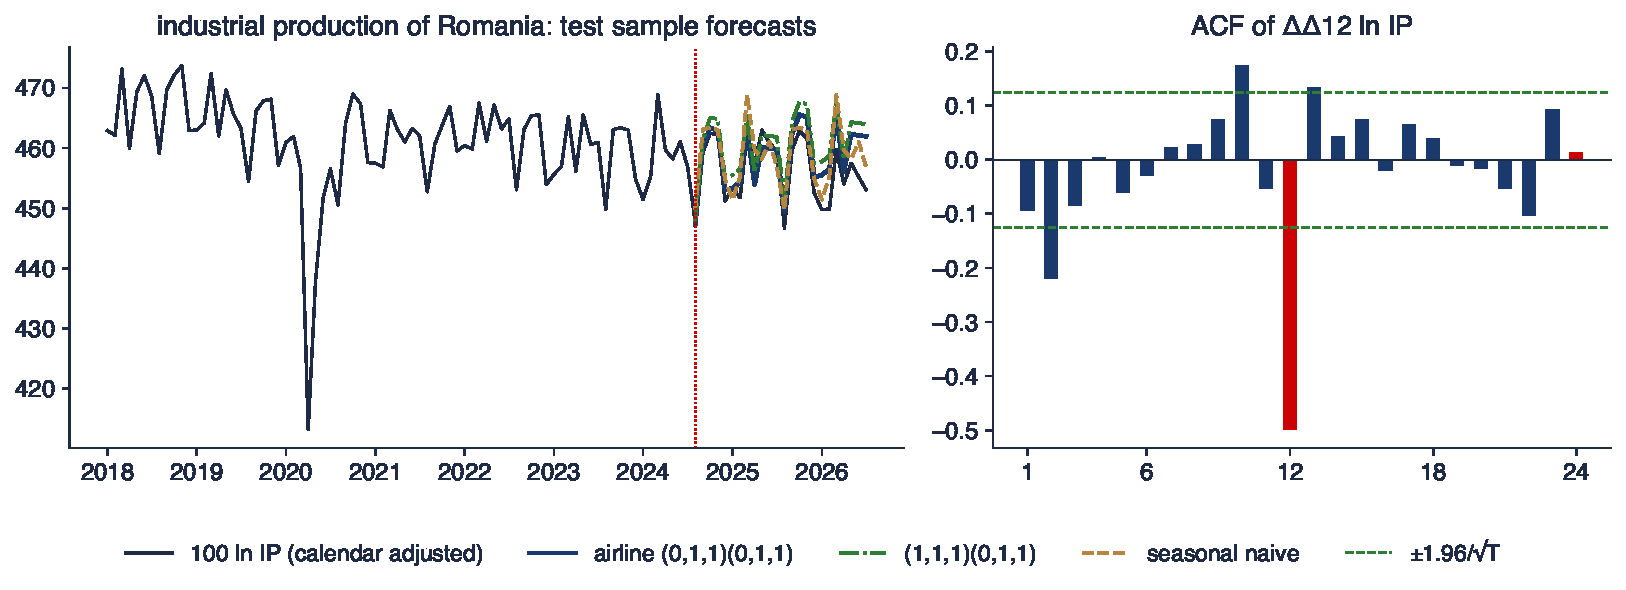
\includegraphics[width=0.96\textwidth,height=0.36\textheight,keepaspectratio]{ch15_sem_b1.pdf}
\end{center}
\vspace{-2mm}
\begin{center}
\scriptsize
\begin{tabular}{lccccc}
\toprule
\textbf{Modelul} & AICc & BIC & LB(12) $p$ & LB(24) $p$ & RMSE test \\
\midrule
airline $(0,1,1)(0,1,1)_{12}$ & 1304{,}2 & 1314{,}3 & 0{,}065 & 0{,}432 & 3{,}75 \\
$(1,1,1)(0,1,1)_{12}$ & 1291{,}1 & 1304{,}5 & 0{,}789 & 0{,}972 & 5{,}29 \\
naiv sezonier & & & & & 3{,}85 \\
\bottomrule
\end{tabular}
\end{center}
\begin{itemize}
    \item Teste: ADF $\tau = \ensuremath{-}1{,}31$ ($p = 0{,}885$) și KPSS 0{,}523 $>$ 0{,}146 pentru nivel; $z_t$: ADF $\ensuremath{-}6{,}47$, KPSS 0{,}055: $d = D = 1$; ACF a lui $z_t$: $\ensuremath{-}0{,}09$; $\ensuremath{-}0{,}22$ la decalajele 1, 2; $\ensuremath{-}0{,}50$ la 12
    \item Airline: $\hat\theta = \ensuremath{-}0{,}205$, $\hat\Theta = \ensuremath{-}0{,}934$; modelul $(1,1,1)$: $\hat\phi = 0{,}574$, $\hat\theta = \ensuremath{-}0{,}828$, factori care aproape se anulează
    \item Interpretare: modelul $(1,1,1)$ cîștigă în eșantion (BIC, reziduuri curate), dar pierde în afara eșantionului; modelul airline este puțin mai bun decît metoda naivă sezonieră: folosim modelul airline și păstrăm metoda naivă sezonieră ca reper
\end{itemize}\quantlet{TSA\_ch15\_seminar}{\qlurl{TSA_ch15_seminar}}
\end{frame}

\begin{frame}{B2: volatilitatea BET din 2015 [Propus]}
\itemsize{\footnotesize}
\begin{itemize}
\item \textbf{Întrebarea}: este bursa de la București azi mai liniștită sau mai agitată decît de obicei și ce înseamnă acest lucru pentru VaR 1\% de mîine? Model: Seminarul 5, B1.
\item \textbf{Date}: randamentele logaritmice zilnice ale BET în \%, ianuarie 2015 -- septembrie 2026 ($n = 2\,925$)
\item \textbf{Cerințe}
\begin{enumerate}
    \item Aplicați testul ARCH-LM cu cinci decalaje pe randamentele centrate.
    \item Estimați un GARCH(1,1) cu inovații Student-$t$; raportați persistența și timpul de înjumătățire.
    \item Comparați volatilitatea anualizată pe termen lung, cea de selecție și cea de azi.
    \item Calculați VaR 1\% de mîine cu cuantila $t$ și cu cea Normală.
    \item Interpretare: este BET azi mai liniștit sau mai agitat decît de obicei?
\end{enumerate}
\item \textbf{Raportați}: un test, cinci parametri, trei volatilități, două valori VaR și o frază
\item Notebook: secțiunea B2
\end{itemize}
\end{frame}

\ifsolutions
\begin{frame}{B2: rezolvare [Propus]}
\itemsize{\footnotesize}
\begin{itemize}
    \item ARCH-LM(5) $= 366{,}8$, $p$ $<$\,0{,}001: efecte ARCH puternice
    \item GARCH(1,1)-$t$: $\mu = 0{,}087$, $\omega = 0{,}069$, $\alpha = 0{,}185$, $\beta = 0{,}740$, $\nu = 5{,}01$; persistența 0{,}925, timpul de înjumătățire 8{,}8 zile
    \item Volatilitatea: pe termen lung 15{,}1\%, de selecție 15{,}5\%, azi 25{,}5\% pe an
    \item VaR 1\% pentru mîine: 4{,}11\% cu cuantila $t$, 3{,}66\% cu cea Normală
    \item Interpretare: azi BET este mai agitat decît de obicei (25{,}5\%, față de 15{,}1\%); cu un timp de înjumătățire de circa 8{,}8 zile, excesul se stinge în cîteva săptămîni; pînă atunci VaR este peste nivelul lui mediu
\end{itemize}\quantlet{TSA\_ch15\_seminar}{\qlurl{TSA_ch15_seminar}}
\end{frame}
\fi

\begin{frame}{B3: randamentele la 10 ani ale României și Germaniei [Propus]}
\itemsize{\footnotesize}
\begin{itemize}
\item \textbf{Întrebarea}: este randamentul la 10 ani al României legat pe termen lung de cel al Germaniei? Model: Seminarul 7, B1 și A3.
\item \textbf{Date}: medii lunare ale randamentelor zilnice la 10 ani (\%), ianuarie 2008 -- septembrie 2026 ($T = 224$)
\item \textbf{Cerințe}
\begin{enumerate}
    \item Aplicați ADF pentru ambele randamente și pentru diferențele lor.
    \item Aplicați testul Engle--Granger (România în funcție de Germania) și raportați $\hat\beta$.
    \item Aplicați testele Johansen ale urmei și ale valorii proprii maxime.
    \item Estimați ecuația cu corecția erorii pentru fiecare randament și calculați timpul de înjumătățire.
    \item Interpretare: este randamentul României legat de cel al Germaniei?
\end{enumerate}
\item \textbf{Raportați}: patru rezultate ADF, două teste de cointegrare, doi coeficienți de ajustare și o frază
\item Notebook: secțiunea B3
\end{itemize}
\end{frame}

\ifsolutions
\begin{frame}{B3: rezolvare [Propus]}
\itemsize{\scriptsize}
\begin{itemize}
    \item ADF: niveluri $\ensuremath{-}2{,}25$ ($p = 0{,}189$) și $\ensuremath{-}1{,}97$ ($p = 0{,}298$): $I(1)$; diferențe $\ensuremath{-}4{,}08$ și $\ensuremath{-}6{,}38$: staționare
    \item Engle--Granger: $\tau = \ensuremath{-}4{,}23 < \ensuremath{-}3{,}36$ ($p = 0{,}003$): cointegrate; $\hat y^{RO} = 3{,}92 + 1{,}35\,y^{DE}$
    \item Johansen: urma 15{,}87 $>$ 15{,}49 ($r = 0$ respins, la limită), 2{,}03 $<$ 3{,}84; valoarea proprie maximă 13{,}84 $<$ 14{,}26: nu se respinge
    \item ECM: România $\gamma = \ensuremath{-}0{,}036$ ($t = \ensuremath{-}1{,}87$), timpul de înjumătățire 19 luni; Germania $\gamma = 0{,}021$ ($t = 2{,}00$); pe termen scurt $\Delta y^{RO}$ în funcție de $\Delta y^{DE}$: 0{,}284 ($t = 2{,}29$)
    \item Interpretare: o legătură pe termen lung slabă și lentă: spread-ul (media 4{,}45 pp) revine la echilibru în cîțiva ani, $\hat\beta > 1$ înseamnă că randamentele României se mișcă mai mult decît cele ale Germaniei; dovezile depind de test, deci răspunsul onest este „probabil, dar slab”
\end{itemize}\quantlet{TSA\_ch15\_seminar}{\qlurl{TSA_ch15_seminar}}
\end{frame}
\fi


%=============================================================================
\section{Partea C: o idee deschisă și critica unui răspuns AI}
%=============================================================================

\begin{frame}{C1: o competiție de prognoză pentru inflația din România [Propus]}
\itemsize{\footnotesize}
\begin{itemize}
\item \textbf{Întrebarea}: ce metodă ar fi prognozat cel mai bine inflația lunară din România în ultimii zece ani, cu o lună și cu douăsprezece luni înainte?
\item \textbf{Date}: IAPC al României (Eurostat), lunar, 2005--2026; Cursul 15 aplică un singur SARIMA pe un singur eșantion de test
\item \textbf{Cerințe}
\begin{enumerate}
    \item Enumerați cinci concurenți: naiv sezonier, SES, SARIMA, ARFIMA, un model ridge cu decalaje și variabile dummy pentru luni.
    \item Descrieți o schemă cu origini mobile: prima origine, pasul, orizonturile, reestimările.
    \item Precizați cum ați trata modificările de taxe din 2010, 2015 și 2025.
    \item Alegeți măsurile de eroare și testul pentru comparație.
\end{enumerate}
\item \textbf{Raportați}: un plan de o pagină pe care o echipă îl poate transforma în proiect
\item Notebook: secțiunea C1
\end{itemize}
\end{frame}

\ifsolutions
\begin{frame}{C1: un plan de referință [Propus]}
\itemsize{\footnotesize}
\begin{itemize}
    \item Origini lunare din ianuarie 2015; orizonturile 1 și 12; fiecare model reestimat la fiecare origine, cu ordinele alese pe datele dinaintea originii
    \item Modificările de taxe: variabile dummy cunoscute dinainte (datele TVA sînt anunțate) sau o funcție de pierdere robustă; raportăm rezultatele cu și fără lunile cu modificări de taxe
    \item MASE față de metoda naivă sezonieră; Diebold--Mariano cu corecția HLN pentru fiecare pereche; un tabel pe orizonturi
    \item Rezultatul așteptat: cîștiguri mici la o lună, aproape niciunul la douăsprezece luni; ARFIMA și SARIMA apropiate; o combinație greu de depășit
\end{itemize}
\end{frame}
\fi

\begin{frame}{C2: verificați un răspuns AI [Propus]}
\itemsize{\scriptsize}
\begin{itemize}
    \item Un student a cerut unui asistent AI să verifice răspunsurile la Partea A. Răspunsul:
    \item \aiprompt{(a) Pentru rata șomajului, ADF dă p = 0{,}52, deci rădăcina unitară se respinge la 5\%.}
    \item \aiprompt{(b) KPSS = 1{,}04 > 0,463 respinge, deci nivelul șomajului este staționar.}
    \item \aiprompt{(c) Pentru DAX, alpha + beta = 0{,}992, deci un șoc se înjumătățește în 1/(1 - 0{,}992) = 128 de zile.}
    \item \aiprompt{(d) VaR 99\% al DAX pentru mîine este -2{,}31\%.}
    \item \aiprompt{(e) Inflația cauzează Granger ROBOR (p = 0{,}036), ceea ce dovedește că inflația determină banca centrală să crească dobînzile.}
    \item \aiprompt{(f) Ljung-Box Q(12) pe reziduurile unui model AR(1) x SAR(1) are 12 grade de libertate.}
    \item Cerințe
    \begin{itemize}
        \item 1. Pentru fiecare afirmație, precizați dacă este corectă; dacă nu este, formulați afirmația corectă și dați valoarea corectă (notebook, secțiunea C2).
        \item 2. Raportați: șase verdicte, fiecare cu un rînd de justificare.
    \end{itemize}
\end{itemize}
\end{frame}

\ifsolutions
\begin{frame}{C2: rezolvare [Propus]}
\itemsize{\footnotesize}
\begin{itemize}
    \item (a) Greșit: $p = 0{,}52 > 0{,}05$: rădăcina unitară nu se respinge; $u_t \sim I(1)$
    \item (b) Greșit: la KPSS, $H_0$ este staționaritatea; respingerea ei indică o rădăcină unitară
    \item (c) Greșit: $h_{1/2} = \ln 0{,}5/\ln 0{,}992 = 88$ de zile; $1/(1 - \alpha - \beta)$ nu este un timp de înjumătățire
    \item (d) Greșit de două ori: nivelul este probabilitatea cozii, VaR 1\%, iar VaR este o pierdere pozitivă: 2{,}31\%
    \item (e) Greșit: cauzalitatea Granger înseamnă predictibilitate suplimentară, nu dovada unui efect cauzal al politicii
    \item (f) Greșit: $12 - 2 = 10$ grade de libertate (doi parametri ARMA estimați)
\end{itemize}\quantlet{TSA\_ch15\_seminar}{\qlurl{TSA_ch15_seminar}}
\end{frame}
\fi


%=============================================================================
\section{Încheiere}
%=============================================================================

\begin{frame}{Idei de reținut}
\itemsize{\small}
\begin{itemize}
    \item Orice problemă de examen are trei părți: formula cu cifrele înlocuite, rezultatul cu unitate și semn, interpretarea
    \item Testele: precizați întîi $H_0$; ADF și KPSS au ipoteze nule opuse; Ljung--Box pe reziduuri pierde $k$ grade de libertate
    \item Prognozele de mînă: scrieți modelul pentru $z_t$, înlocuiți ultimele valori, apoi refaceți diferențierile
    \item Un model mai bun în eșantion nu prognozează neapărat mai bine (B1); judecați-l pe un eșantion de test, față de un reper
    \item Un răspuns AI este o ciornă: verificați ipotezele nule, timpul de înjumătățire, nivelul VaR și gradele de libertate
\end{itemize}
\end{frame}

\begin{frame}{După seminar}
\itemsize{\small}
\begin{itemize}
    \item Cursul 15 adună întreaga materie: harta cursului, cîte un slide de recapitulare pentru fiecare capitol, trusa de instrumente, Box--Jenkins pe inflația din România, opt probleme de tip examen rezolvate, proiectul
    \item Încercați cerințele [Propus] întîi pe hîrtie, apoi verificați-le în notebook
    \item C1 poate deveni un proiect de echipă
    \item Lectură: \refHP; \refFPP; \refBJ
    \item \textbf{Seminarul are rol de exercițiu și nu se notează; rezolvările cerințelor [Propus] se discută la seminar}
\end{itemize}
\end{frame}


%=============================================================================
\section{Bibliografie}
%=============================================================================

\begin{frame}{Bibliografie}
\itemsize{\tiny}
\begin{itemize}
    \item Bollerslev, T. (1986). Generalized autoregressive conditional heteroskedasticity. \textit{Journal of Econometrics}, 31(3), 307--327. \href{https://doi.org/10.1016/0304-4076(86)90063-1}{doi:10.1016/0304-4076(86)90063-1}
    \item Box, G. E. P., Jenkins, G. M., \& Reinsel, G. C. (2008). \textit{Time Series Analysis: Forecasting and Control} (4th ed.). Wiley. \href{https://doi.org/10.1002/9781118619193}{doi:10.1002/9781118619193}
    \item Dickey, D. A., \& Fuller, W. A. (1979). Distribution of the estimators for autoregressive time series with a unit root. \textit{Journal of the American Statistical Association}, 74(366), 427--431. \href{https://doi.org/10.1080/01621459.1979.10482531}{doi:10.1080/01621459.1979.10482531}
    \item Diebold, F. X., \& Mariano, R. S. (1995). Comparing predictive accuracy. \textit{Journal of Business \& Economic Statistics}, 13(3), 253--263. \href{https://doi.org/10.1080/07350015.1995.10524599}{doi:10.1080/07350015.1995.10524599}
    \item Engle, R. F., \& Granger, C. W. J. (1987). Co-integration and error correction: Representation, estimation, and testing. \textit{Econometrica}, 55(2), 251--276. \href{https://doi.org/10.2307/1913236}{doi:10.2307/1913236}
    \item Granger, C. W. J. (1969). Investigating causal relations by econometric models and cross-spectral methods. \textit{Econometrica}, 37(3), 424--438. \href{https://doi.org/10.2307/1912791}{doi:10.2307/1912791}
    \item Huang, C., \& Petukhina, A. (2022). \textit{Applied Time Series Analysis and Forecasting with Python}. Springer. \href{https://doi.org/10.1007/978-3-031-13584-2}{doi:10.1007/978-3-031-13584-2}
    \item Hyndman, R. J., \& Athanasopoulos, G. (2021). \textit{Forecasting: Principles and Practice} (3rd ed.). OTexts. \href{https://otexts.com/fpp3/}{otexts.com/fpp3}
    \item Johansen, S. (1991). Estimation and hypothesis testing of cointegration vectors in Gaussian vector autoregressive models. \textit{Econometrica}, 59(6), 1551--1580. \href{https://doi.org/10.2307/2938278}{doi:10.2307/2938278}
    \item Kwiatkowski, D., Phillips, P. C. B., Schmidt, P., \& Shin, Y. (1992). Testing the null hypothesis of stationarity against the alternative of a unit root. \textit{Journal of Econometrics}, 54(1--3), 159--178. \href{https://doi.org/10.1016/0304-4076(92)90104-Y}{doi:10.1016/0304-4076(92)90104-Y}
    \item Ljung, G. M., \& Box, G. E. P. (1978). On a measure of lack of fit in time series models. \textit{Biometrika}, 65(2), 297--303. \href{https://doi.org/10.1093/biomet/65.2.297}{doi:10.1093/biomet/65.2.297}
\end{itemize}
\end{frame}

\end{document}
